\documentclass{article}
\usepackage[utf8]{inputenc}
\usepackage{graphicx}
\usepackage{float}
\usepackage{amsmath}
\usepackage{multirow}
\usepackage{longtable}


\title{Laboratorio di Sistemi Meccatronici 2 \\
       Progetto: Macchina laser 2gld}
\author{Raul Luizaga \\ Stefano Rubis}
\date{December 2021}


\begin{document}

\maketitle

\begin{figure}[H]
\centering
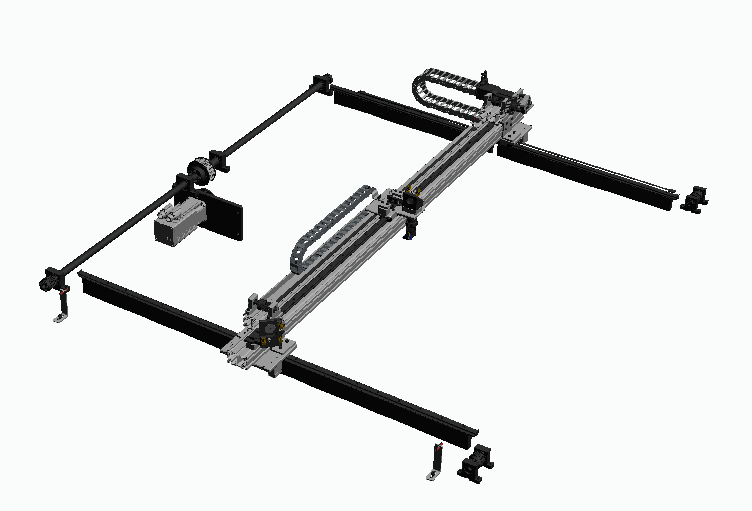
\includegraphics[width=.6\textwidth]{asse.png}
\end{figure}

\section{Introduction}
Il progetto è stato sviluppato in due fasi: la prima svolta da casa e la seconda in laboratorio. Nello specifico possiamo trovare 5 sottofasi: 
\begin{enumerate}
\item Modellazione dei singoli assi tenendo conto anche dell'elasticità delle cinghie, ricreando il noto sistema massa-carrello
\item  Sintesi del regolatore di posizione del singolo asse (controllo classico, controllo moderno)
\item Simulazione in ambiente Simulink del comportamento dei singoli assi
\item Definizione della strategia di percorrenza delle traiettorie
\item  Simulazione percorrenza traiettorie
\end{enumerate}

\section{Modellazione dei singoli assi}

\subsection{Modellazione ASSE X} 

\begin{figure}[H]
\centering
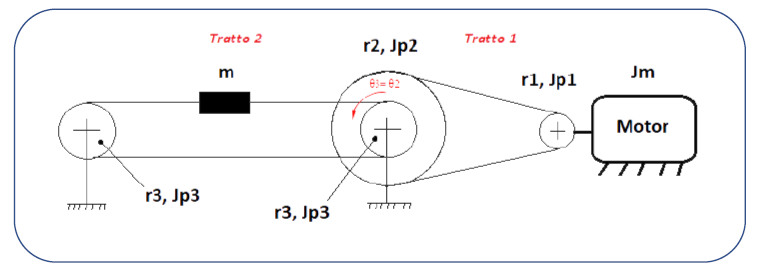
\includegraphics[width=.6\textwidth]{./assex/assex.png}
\end{figure}
La trasmissione del moto è definita da 4 pulegge, ognuna con un proprio raggio $R_{i}$ ed una propria inerzia $J_{i}$. La modellazione è avvenuta tramite equazioni di Lagrange e di conseguenza si sono dovute scegliere le coordinate libere che nel nostro caso sono $x$,$\theta_{1}$,$\theta_{2}$,$\theta_{3}$. 
Questi valori corrispondono alle rotazioni delle pulegge. L'albero di collegamento fra il primo ed il secondo tratto può essere considerato rigido. Per semplificare il problema, abbiamo studiato il caso suddividendolo in due tratti:
\begin{itemize}

\item tratto 1: comprende le coordinate libere $\theta_{1},\theta_{2}$
\item tratto 2: comprende le coordinate libere $x,\theta_{2},\theta_{3}$
\end{itemize}

Equazione di Lagrange: 
\begin{equation*}
\frac{\partial }{\partial t}(\frac{\partial T} {\partial \dot{q}}) - (\frac{\partial T}{\partial q}) + \frac{\partial U}{\partial q} + \frac{\partial D}{\partial \dot{q}} = Q_i
\end{equation*}
%                                                           INIZIO TRATTO 1
\subsection{Modellazione ASSE X - Tratto 1} 
\begin{figure}[H]
\centering
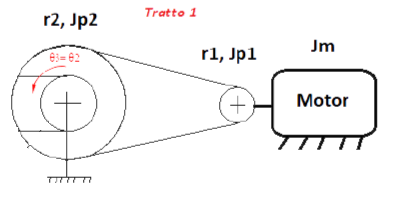
\includegraphics[width=.6\textwidth]{./assex/tratto1.png}
\end{figure}
$T = T_{puleggia_1} + T_{puleggia_2}+ T_{motore}
= {1 \over 2}J_{p_1}\dot{\theta_{1}}^{2}+ {1 \over 2}J_{p_2}\dot{\theta_{2}}^{2} + {1 \over 2}J_{m}\dot{\theta_{1}}^{2}$
\\
\\
$U = U_{gravitazionale} + U_{cinghie}
=  2[ {1 \over 2}k _{1}(\theta_{2}R_{2}-\theta_{1}R_{1})^{2} ]$
\\
\\
$D = 2[ {1 \over 2}c _{1}(\dot{\theta_{2}} R_{2}-\dot{\theta_{1}}R_{1})^{2} ]$
\\
\\
%                                            INIZIO EQUAZIONI DI LAGRANGE PER LA COORDINATA THETA1 
Coordinata libera $\theta_{1}$:
\\
\\

\begin{equation*}
{ \partial T \over \partial \theta_{1}} = 0 ; { \partial T \over \partial   \dot{\theta_{1}} } = 0;  \frac{\partial }{\partial T}(\frac{\partial T}{\partial \dot{\theta_{1}}})  = \ddot{\theta_{1}}(J_{p1} + J_{m})
\end{equation*} 
\begin{equation*}
\frac{\partial U}{\partial \theta_{1}} = -2k_{1}R_{1}(\theta_{2}R_{2} - \theta_{1}R_{1});
\frac{\partial D}{\partial \dot{\theta_{1}}} = -2c_{1}R_{1}(\dot{(\theta_{2}}R_{2} - \dot{(\theta_{1}}R_{1})
\end{equation*}
\\
% PRIMA EQUAZIONE DEL TRATTO 1
Da cui ottengo la prima equazione: 
\\
\begin{equation*}
 \ddot{\theta_{1}}(J_{p1}+J_{m}) - R_{1}[2k_{1}(\theta_{2}R_{2}-\theta_{1}R_{1})+ 2c_{1}(\dot{\theta_{2}}R_{2}-\dot{\theta_{1}}R_{1})] = Q_{\theta_1}
\end{equation*}
\\
%                                           INIZIO EQUAZIONI DI LAGRANDE PER LA COORDINATA THETA2 
Coordinata libera $\theta_{2}$:
\\
\\
\begin{equation*}
{ \partial T \over \partial \theta_{2}} = 0 ; { \partial T \over \partial   \dot{\theta_{2}} } = \dot{\theta_{2}}J_{p2};  \frac{d}{dT}(\frac{\partial T}{\partial \dot{\theta_{2}}})  = \ddot{\theta_{2}}J_{p2}
\end{equation*}

\begin{equation*}
\frac{\partial U}{\partial \theta_{2}} = 2k_{1}R_{2}(\theta_{2}R_{2} - \theta_{1}R_{1})
\frac{\partial D}{\partial \dot{\theta_{2}}} = 2c_{1}R_{2}(\dot{\theta_{2}}R_{2} - \dot{\theta_{1}}R_{1})
\end{equation*}
\\
%                                            SECONDA EQUAZIONE DEL TRATTO 1
Da cui ottengo la seconda equazione: 
\\
\begin{equation*}
 \ddot{\theta_{2}}(J_{p2}) + R_{2}[2k_{1}(\theta_{2}R_{2}-\theta_{1}R_{1})+ 2c_{1}(\dot{\theta_{2}}R_{2}-\dot{\theta_{1}}R_{1})] = Q_{\theta_2}
\end{equation*}
\\
ricapitolando ottendo un sistema di due equazioni:
\begin{equation*}
\begin{cases}
\ddot{\theta_{1}}(J_{p1}+J_{m}) - R_{1}[2k_{1}(\theta_{2}R_{2}-\theta_{1}R_{1})+ 2c_{1}(\dot{\theta_{2}}R_{2}-\dot{\theta_{1}}R_{1})] = Q_{\theta_1}\\
\ddot{\theta_{2}}(J_{p2}) + R_{2}[2k_{1}(\theta_{2}R_{2}-\theta_{1}R_{1})+ 2c_{1}(\dot{\theta_{2}}R_{2}-\dot{\theta_{1}}R_{1})] = Q_{\theta_2}
\end{cases}
\end{equation*}


%                                                           INIZIO TRATTO 2
\subsection{Modellazione ASSE X - Tratto 2} 
\begin{figure}[H]
\centering
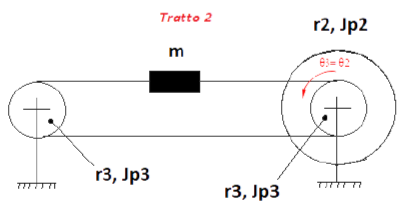
\includegraphics[width=.6\textwidth]{./assex/tratto2.png}
\end{figure}

$T = T_{carrello} + T_{puleggia_2}+ T_{puleggia_3}
= {1 \over 2}J_{p_3}\dot{\theta_{3}}^{2}+ {1 \over 2}m\dot{x}^{2} + {1 \over 2}J_{p_3}\dot{\theta_{2}}^{2}$
\\
\\
$U = U_{gravitazionale} + U_{cinghie} $
\\
$ ={1\over 2}k_{3}(x)(x-\theta_{3}R_{3})^{2}+\frac{1}{2}k_{2}(x)(x-\theta_{2}R_{3})^{2}+{1 \over 2}k_{4}(R_{3}\theta{2}-R_{3}\theta{3})^{2}$
\\
\\
$D ={1\over 2}c_{3}(x)(\dot{x}-\dot{\theta_{3}}R_{3})^{2}+\frac{1}{2}c_{2}(x)(\dot{x}-\dot{\theta_{2}}R_{3})^{2}+{1\over2} c_{4}(R_{3}\dot{\theta{2}}-R_{3}\dot{\theta{3}})^{2}$
\\
\\
Nota: 
$$c_{2}(x), c_{3}(x),k_{2}(x), k_{3}(x)$$ sono variabili.
\\
\\
Per una maggiore semplicità descrittiva, possiamo utilizzare la notazione:
\begin{equation*}
c_{2}(x) = c_{2};
c_{3}(x) = c_{3};
k_{2}(x) = k_{2};
k_{3}(x) = k_{3};
\end{equation*}
\\
%                                            INIZIO EQUAZIONI DI LAGRANDE PER LA COORDINATA X 
Coordinata libera $x$:
\\
\\
\begin{equation*}
\frac{ \partial T}{\partial x} = 0 ; \frac{\partial T}{\partial \dot{x}} = m\dot{x};  \frac{\partial}{\partial T}(\frac{\partial T}{\partial \dot{x}})  = \ddot{x}m;
\end{equation*}
\\
\\
\begin{equation*}
\frac{\partial U}{\partial x} = k_3(x-\theta_3R_3) + k_2(x -\theta_2R_3)
\end{equation*}
\\
\\
\begin{equation*}
\frac{\partial D}{\partial \dot{x}} = c_3(\dot{x}-\dot{\theta_3}R_3) + c_2(\dot{x} -\dot{\theta_2}R_3)
\end{equation*}
\\
% PRIMA EQUAZIONE DEL TRATTO 2
Da cui ottengo la prima equazione: 
\\
\begin{equation*}
 \ddot{x}m + k_{3}(x-\theta_{3}R_{3}) + k_{2}(x- \theta_{2}R_{3})+ c_{3}(\dot{x}-\dot{\theta_3}R_{3}) + c_{2}(\dot{x} - \dot{\theta_{2}}R_{3}) = Q_x
\end{equation*}
\\
%                                            INIZIO EQUAZIONI DI LAGRANDE PER LA COORDINATA THETA2 
Coordinata libera $\theta_2$:
\\
\\
\begin{equation*}
\frac{ \partial T}{\partial \theta_2} = 0 ; \frac{\partial T}{\partial \dot{\theta_2}} = J_{p_3}\dot{\theta_2};  \frac{d}{dT}(\frac{\partial T}{\partial \dot{\theta_2}})  = \ddot{\theta_2}J_{p_3}
\end{equation*}
\\
\\
\begin{equation*}
\frac{\partial U}{\partial \theta_2} = -k_2R_3(x-\theta_2R_3) + k_4R_3(\theta_2 R_3 - \theta_3 R_3)
\end{equation*}
\\
\\
\begin{equation*}
\frac{\partial D}{\partial \dot{x}} = -c_2R_3(\dot{x} - \dot{\theta_2}R_3) - c_4R_3(\dot{\theta_2}R_3 - \dot{\theta_3}R_3)
\end{equation*}
\\
% SECONDA EQUAZIONE DEL TRATTO 2
Da cui ottengo la seconda equazione: 
\\
\begin{equation*}
 \ddot{\theta_2}J_{p_3} - k_{2}R_{3}(x - \theta_{2}R_{3}) + k_{4}R_3(\theta_{2}R_3 - \theta_{3}R_{3}) - c_{2}R_{3}(\dot{x}-\dot{\theta_2}R_{3}) + c_{4}R_{3}(\dot{\theta_2}R_3 - \dot{\theta_{3}}R_{3}) = Q_{\theta_2}
\end{equation*}
%                                            INIZIO EQUAZIONI DI LAGRANDE PER LA COORDINATA THETA3
Coordinata libera $\theta_3$:
\\
\\
\begin{equation*}
\frac{ \partial T}{\partial \theta_3} = 0 ; \frac{\partial T}{\partial \dot{\theta_3}} = J_{p_3}\dot{\theta_3};  \frac{d}{dT}(\frac{\partial T}{\partial \dot{\theta_3}})  = \ddot{\theta_3}J_{p_3}
\end{equation*}
\\
\\
\begin{equation*}
\frac{\partial U}{\partial \theta_3} = -k_3R_3(x - \theta_3R_3) - k_4R_3(\theta_2 R_3 - \theta_3 R_3)
\end{equation*}
\\
\\
\begin{equation*}
\frac{\partial D}{\partial \dot{x}} = -c_3R_3(\dot{x}-\dot{\theta_3}R_3) - c_4R_3(\dot{\theta_2} R_3 - \dot{\theta_3} R_3)
\end{equation*}
\\
% TERZA EQUAZIONE DEL TRATTO 2
Da cui ottengo la terza equazione: 
\\
\begin{equation*}
 \ddot{\theta_3}J_{p_3} - k_{3}R_{3}(x - \theta_{3}R_{3}) - k_{4}R_3(\theta_{2}R_3 - \theta_{3}R_{3}) - c_{3}R_{3}(\dot{x}-\dot{\theta_3}R_{3}) - c_{4}R_{3}(\dot{\theta_2}R_3 - \dot{\theta_{3}}R_{3}) = Q_{\theta_3}
\end{equation*}
\\
Ricapitolando ottengo un sistema di 3 equazioni:
\begin{equation*}
\begin{cases}
 \ddot{x}m + k_{3}(x-\theta_{3}R_{3}) + k_{2}(x- \theta_{2}R_{3})+ c_{3}(\dot{x}-\dot{\theta_3}R_{3}) + c_{2}(\dot{x} - \dot{\theta_{2}}R_{3}) = Q_x\\
 \ddot{\theta_3}J_{p_3} - k_{3}R_{3}(x - \theta_{3}R_{3}) - k_{4}R_3(\theta_{2}R_3 - \theta_{3}R_{3}) - c_{3}R_{3}(\dot{x}-\dot{\theta_3}R_{3}) - c_{4}R_{3}(\dot{\theta_2}R_3 - \dot{\theta_{3}}R_{3}) = Q_{\theta_3}\\
 \ddot{\theta_2}J_{p_3} - k_{2}R_{3}(x - \theta_{2}R_{3}) + k_{4}R_3(\theta_{2}R_3 - \theta_{3}R_{3}) - c_{2}R_{3}(\dot{x}-\dot{\theta_2}R_{3}) + c_{4}R_{3}(\dot{\theta_2}R_3 - \dot{\theta_{3}}R_{3}) = Q_{\theta_2}
\end{cases}
\end{equation*}
%                                                   TRATTO 1-2
\subsection{Modellazione ASSE X  Tratto 1-2} 
Unione dei 2 sotto-modelli:
\begin{equation*}
\begin{cases}
    %x
\ddot{x}m + k_{3}(x-\theta_{3}R_{3}) + k_{2}(x- \theta_{2}R_{3})+ c_{3}(\dot{x}-\dot{\theta_3}R_{3}) + c_{2}(\dot{x} - \dot{\theta_{2}}R_{3}) = 0\\
    %theta1
\ddot{\theta_{1}}(J_{p1}+J_{m}) - R_{1}[2k_{1}(\theta_{2}R_{2}-\theta_{1}R_{1})+ 2c_{1}(\dot{\theta_{2}}R_{2}-\dot{\theta_{1}}R_{1})] = C_{m}\\
    %theta2
\ddot{\theta_{2}}(J_{p2} + J_{p_3} + R_{2}[2k_{1}(\theta_{2}R_{2}-\theta_{1}R_{1})+ 2c_{1}(\dot{\theta_{2}}R_{2}-\dot{\theta_{1}}R_{1})]+ \\ - k_{2}R_{3}(x - \theta_{2}R_{3}) + k_{4}R_3(\theta_{2}R_3 - \theta_{3}R_{3}) - c_{2}R_{3}(\dot{x}-\dot{\theta_2}R_{3}) + c_{4}R_{3}(\dot{\theta_2}R_3 - \dot{\theta_{3}}R_{3}) = 0\\
 %theta3
 \ddot{\theta_3}J_{p_3} - k_{3}R_{3}(x - \theta_{3}R_{3}) - k_{4}R_3(\theta_{2}R_3 - \theta_{3}R_{3}) - c_{3}R_{3}(\dot{x}-\dot{\theta_3}R_{3}) - c_{4}R_{3}(\dot{\theta_2}R_3 - \dot{\theta_{3}}R_{3}) = 0\\
\end{cases}
\end{equation*}
Definisco le matrici M,K,C ed F per esprimere tutto in notazione matriciale:
\\
\\
M= 
$$
\begin{bmatrix}
J_{p_1}+J_m  & 0 & 0 & 0\\
0 & J_{p_2}+J_{p_3} & 0 & 0\\
0 & 0 & J_{p_3} & 0\\
0 & 0 & 0 & m
\end{bmatrix}
$$
K= 
$$
\begin{bmatrix}
 2k_1R_1^2 & -2k_1R_{2}R_{1} & 0 & 0\\
-2k_{1}R_{2}R_{1} & 2k_{1}R_{2}^2 + (k_2+k_4)R_{3}^2  & -k_{4}R_{3}^2 & -k_{2}R_{3}\\
0 & -k_{4}R_{3}^2  & (k_{3}+k_{4})R_{3}^2 & -k_{3}R_{3}\\
0 & -k_{2}R_{3} &  -k_{3}R_{3} & k_{3}+k_{2}
\end{bmatrix}
$$
C= 
$$
\begin{bmatrix}
 2c_{1}R_{1}^2 & -2c_{1}R_{2}R_{1} & 0 & 0\\
-2c_{1}R_{2}R_{1} & 2c_{1}R_{2}^2 + (c_{2}+c_{4})R_{3}^2  & -c_{4}R_{3}^2 & -c_{2}R_{3}\\
0 & -c_{4}R_{3}^2  & (c_{3}+c_{4})R_{3}^2 & -c_{3}R_{3}\\
0 & -c_{2}R_{3} &  -c_{3}R_{3} & c_{3}+c_{2}
\end{bmatrix}
$$
F= 
$$
\begin{bmatrix}
C_m \\
0 \\
0\\
0
\end{bmatrix}
$$
ottengo così la relazione matriciale:


$$ M\ddot{X} + C\dot{X} + KX = F $$
dove:
\\
\\
X= 
$$
\begin{bmatrix}
\theta_1 \\
\theta_2\\
\theta_3\\
x 
\end{bmatrix}
$$
$\dot{X}$= 
$$
\begin{bmatrix}
\dot{\theta_1} \\
\dot{\theta_2}\\
\dot{\theta_3}\\
\dot{x} 
\end{bmatrix}
$$
$\ddot{X}$= 
$$
\begin{bmatrix}
\ddot{\theta_1} \\
\ddot{\theta_2}\\
\ddot{\theta_3}\\
\ddot{x} 
\end{bmatrix}
$$
%---------------------------------- MODELLIZZAZIONE ASSE Y-----------------------------------
\subsection{Modellazione ASSE Y} 

\begin{figure}[H]
\centering
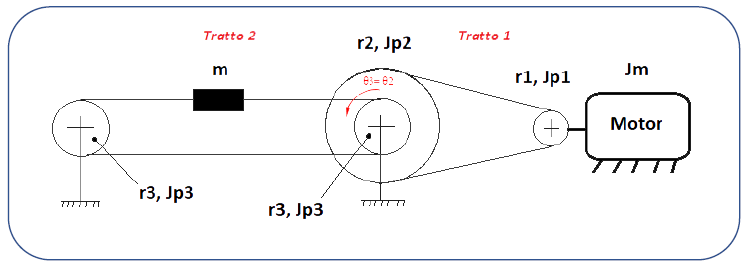
\includegraphics[width=.6\textwidth]{./assey/assey.png}
\end{figure}
Vista del modello completo:
\begin{figure}[H]
\centering
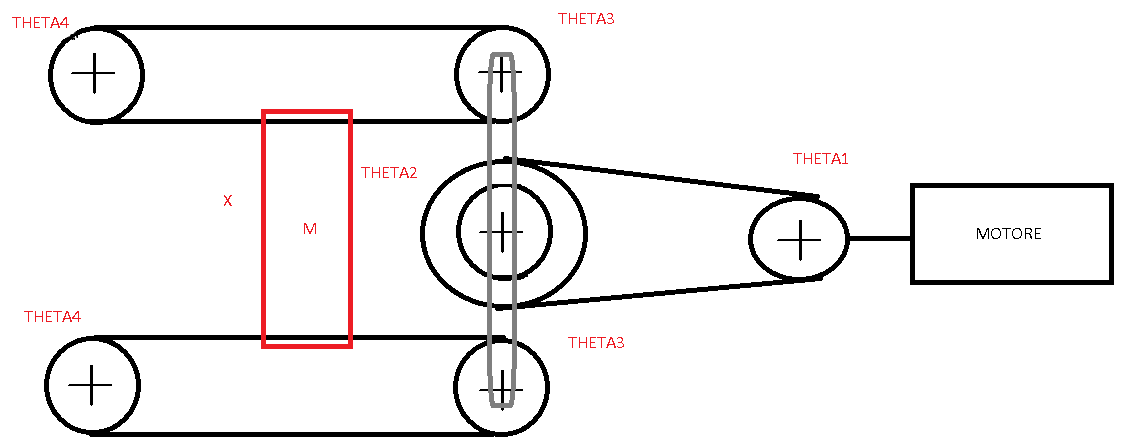
\includegraphics[width=.7\textwidth]{./assey/assey_p.png}
\end{figure}
Faccio 2 osservazioni :
\begin{enumerate}
    \item  Il tratto 2 è simmetrico
    \item Il tratto 1 è identico al tratto 1 del modello dell'asse x
\end{enumerate}
Rappresentazione del modello dell'asse y in modo funzionale:



\begin{figure}[H]
\centering
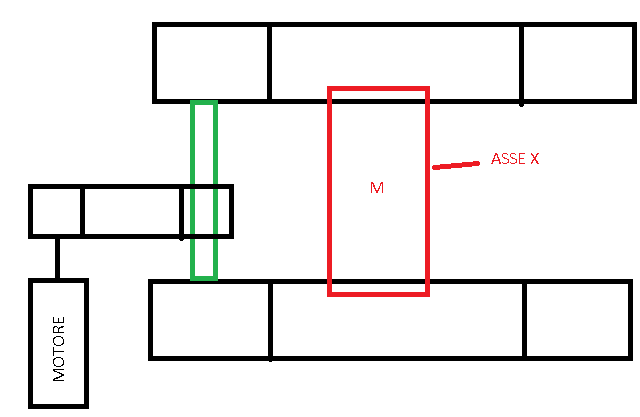
\includegraphics[width=.6\textwidth]{./assey/assey_nf.png}
\end{figure}
Il quale può essere visto anche in questo modo per capire meglio come trattare le rigidezze:
\begin{figure}[H]
\centering
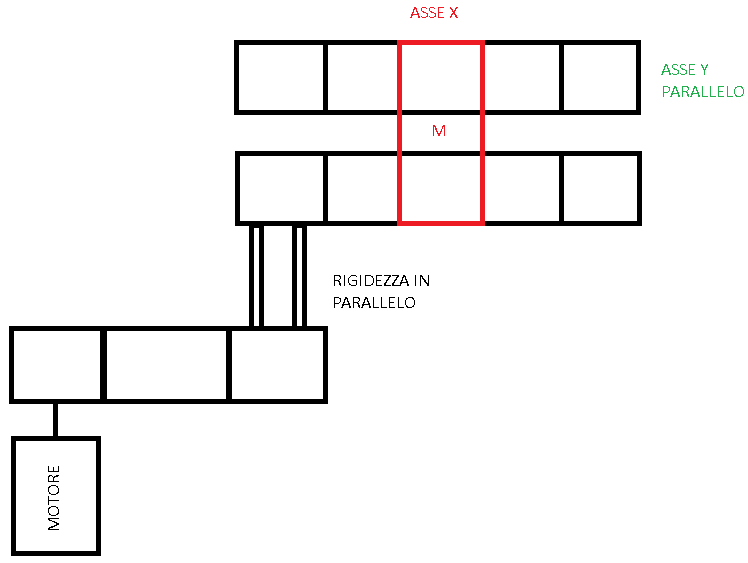
\includegraphics[width=.6\textwidth]{./assey/assey_nfm.png}
\end{figure}
L'asse y è composta da 7 pulegge, ognuna con un proprio raggio $R_{i}$ ed una propria inerzia $J_{i}$. La modellizzazione è avvenuta tramite equazioni di Lagrange e di conseguenza si sono dovute scegliere le coordinate libere che nel nostro caso sono $x,\theta_{1},\theta_{2},\theta_{3} $ e $ \theta_4$. Anche in questo caso per semplificare i conti abbiamo suddivido il problema il due tratti. Come osservato prima il tratto 2 è simmetrico, di conseguenza posso vedere l'asse y composto da 5 pulegge perchè le pulegge: $puleggia_{4}$ e la $puleggia_{3}$ vengono prese 2 volte.
%------------------------- inizio scrittura equazioni-------------------------------
\subsection{Modellazione ASSE Y - Tratto 1} 
\begin{figure}[H]
\centering
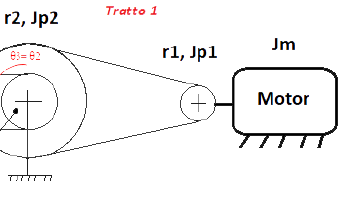
\includegraphics[width=.6\textwidth]{./assey/tratto1.png}
\end{figure}
$T = T_{puleggia_1} + T_{puleggia_2}+ T_{motore}
= {1 \over 2}J_{p_1}\dot{\theta_{1}}^{2}+ {1 \over 2}J_{p_2}\dot{\theta_{2}}^{2} + {1 \over 2}J_{m}\dot{\theta_{1}}^{2}$
\\
\\
$U = U_{gravitazionale} + U_{cinghie}
=  2[ {1 \over 2}k _{1}(\theta_{2}R_{2}-\theta_{1}R_{1})^{2} ]$
\\
\\
$D = 2[ {1 \over 2}c _{1}(\dot{\theta_{2}} R_{2}-\dot{\theta_{1}}R_{1})^{2} ]$
\\
\\
%                                            INIZIO EQUAZIONI DI LAGRANDE PER LA COORDINATA THETA1 
Coordinata libera $\theta_{1}$:
\\
\\

\begin{equation*}
{ \partial T \over \partial \theta_{1}} = 0 ; { \partial T \over \partial   \dot{\theta_{1}} } = 0;  \frac{\partial}{\partial T}(\frac{\partial T}{\partial \dot{\theta_{1}}})  = \ddot{\theta_{1}}(J_{p1} + J_{m})
\end{equation*}
\begin{equation*}
\frac{\partial U}{\partial \theta_{1}} = -2k_{1}R_{1}(\theta_{2}R_{2} - \theta_{1}R_{1});
\frac{\partial D}{\partial \dot{\theta_{1}}} = -2c_{1}R_{1}(\dot{(\theta_{2}}R_{2} - \dot{(\theta_{1}}R_{1})
\end{equation*}
\\
% PRIMA EQUAZIONE DEL TRATTO 1
Da cui ottengo la prima equazione: 
\\
\begin{equation*}
 \ddot{\theta_{1}}(J_{p1}+J_{m}) - R_{1}[2k_{1}(\theta_{2}R_{2}-\theta_{1}R_{1})+ 2c_{1}(\dot{\theta_{2}}R_{2}-\dot{\theta_{1}}R_{1})] = Q_{\theta_1}
\end{equation*}
\\
%                                           INIZIO EQUAZIONI DI LAGRANDE PER LA COORDINATA THETA2 
Coordinata libera $\theta_{2}$:
\\
\\
\begin{equation*}
{ \partial T \over \partial \theta_{2}} = 0 ; { \partial T \over \partial   \dot{\theta_{2}} } = \dot{\theta_{2}}J_{p2};  \frac{\partial}{\partial T}(\frac{\partial T}{\partial \dot{\theta_{2}}})  = \ddot{\theta_{2}}J_{p2}
\end{equation*}

\begin{equation*}
\frac{\partial U}{\partial \theta_{2}} = 2k_{1}R_{2}(\theta_{2}R_{2} - \theta_{1}R_{1})
\frac{\partial D}{\partial \dot{\theta_{2}}} = 2c_{1}R_{2}(\dot{\theta_{2}}R_{2} - \dot{\theta_{1}}R_{1})
\end{equation*}
\\
%                                            SECONDA EQUAZIONE DEL TRATTO 1
Da cui ottengo la seconda equazione: 
\\
\begin{equation*}
 \ddot{\theta_{2}}(J_{p2}) + R_{2}[2k_{1}(\theta_{2}R_{2}-\theta_{1}R_{1})+ 2c_{1}(\dot{\theta_{2}}R_{2}-\dot{\theta_{1}}R_{1})] = Q_{\theta_2}
\end{equation*}
\\
%---------------------------------------------------- EQUAZIONI DEL TRATTO 1-----------------------------------------------------------------------
ricapitolando ottengo un sistema di due equazioni:
\begin{equation*}
\begin{cases}
\ddot{\theta_{1}}(J_{p1}+J_{m}) - R_{1}[2k_{1}(\theta_{2}R_{2}-\theta_{1}R_{1})+ 2c_{1}(\dot{\theta_{2}}R_{2}-\dot{\theta_{1}}R_{1})] = Q_{\theta_1}\\
\ddot{\theta_{2}}(J_{p2}) + R_{2}[2k_{1}(\theta_{2}R_{2}-\theta_{1}R_{1})+ 2c_{1}(\dot{\theta_{2}}R_{2}-\dot{\theta_{1}}R_{1})] = Q_{\theta_2}
\end{cases}
\end{equation*}
%---------------------------------------------------- FINE EQUAZIONI DEL TRATTO 1-----------------------------------------------------------------------
E' identico al tratto-1 dell'asse x.
%                                                           INIZIO TRATTO 2
\subsection{Modellazione ASSE Y - Tratto 2} 
\begin{figure}[H]
\centering
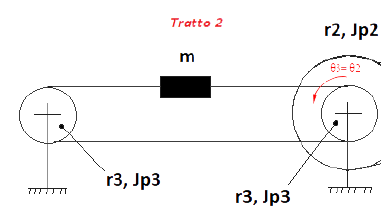
\includegraphics[width=.6\textwidth]{./assey/tratto2.png}
\end{figure}

$T = T_{asse_x} + T_{puleggia_2}+ T_{puleggia_3}
= J_{p_3}\dot{\theta_{3}}^{2}+ J_{p_3}\dot{\theta_{2}}^{2}+ {1 \over 2}m\dot{x}^{2} $
\\
\\
$U = U_{gravitazionale} + U_{cinghie} $
\\
$ =k_{3}(x)(x-\theta_{3}R_{3})^{2}+k_{2}(x)(x-\theta_{2}R_{3})^{2}+k_{4}(R_{3}\theta{2}-R_{3}\theta{3})^{2}$
\\
\\
$D =c_{3}(x)(\dot{x}-\dot{\theta_{3}}R_{3})^{2}+c_{2}(x)(\dot{x}-\dot{\theta_{2}}R_{3})^{2}+ c_{4}(R_{3}\dot{\theta{2}}-R_{3}\dot{\theta{3}})^{2}$
\\
\\
Nota: 
$$c_{2}(x), c_{3}(x),k_{2}(x), k_{3}(x)$$ sono variabili.
\\
\\
Notazione:
\begin{equation*}
c_{2}(x) = c_{2};
c_{3}(x) = c_{3};
k_{2}(x) = k_{2};
k_{3}(x) = k_{3};
\end{equation*}
\\
%                                            INIZIO EQUAZIONI DI LAGRANDE PER LA COORDINATA X 
Coordinata libera $x$:
\\
\\
\begin{equation*}
\frac{ \partial T}{\partial x} = 0 ; \frac{\partial T}{\partial \dot{x}} = \dot{x}m;  \frac{\partial}{\partial T}(\frac{\partial T}{\partial \dot{x}})  = \ddot{x}m;
\end{equation*}
\\
\\
\begin{equation*}
\frac{\partial U}{\partial x} = 2k_3(x-\theta_3R_3) + 2k_2(x -\theta_2R_3)
\end{equation*}
\\
\\
\begin{equation*}
\frac{\partial D}{\partial \dot{x}} = 2c_3(\dot{x}-\dot{\theta_3}R_3) + 2c_2(\dot{x} -\dot{\theta_2}R_3)
\end{equation*}
\\
% PRIMA EQUAZIONE DEL TRATTO 2
Da cui ottengo la prima equazione: 
\\
\begin{equation*}
 \ddot{x}m + 2k_{3}(x-\theta_{3}R_{3}) + 2k_{2}(x- \theta_{2}R_{3})+ 2c_{3}(\dot{x}-\dot{\theta_3}R_{3}) + 2c_{2}(\dot{x} - \dot{\theta_{2}}R_{3}) = Q_x
\end{equation*}
\\
%                                            INIZIO EQUAZIONI DI LAGRANDE PER LA COORDINATA THETA2 
Coordinata libera $\theta_2$:
\\
\\
\begin{equation*}
\frac{ \partial T}{\partial \theta_2} = 0 ; \frac{\partial T}{\partial \dot{\theta_2}} = 2\dot{\theta_2}J_{p_3};  \frac{\partial}{d
\partial T}(\frac{\partial T}{\partial \dot{\theta_2}})  = 2\ddot{\theta_2}J_{p_3}
\end{equation*}
\\
\\
\begin{equation*}
\frac{\partial U}{\partial \theta_2} = -2k_2R_3(x-\theta_2R_3) + 2k_4R_3(\theta_2 R_3 - \theta_3 R_3)
\end{equation*}
\\
\\
\begin{equation*}
\frac{\partial D}{\partial \dot{\theta_2}} = -2c_2R_3(\dot{x} - \dot{\theta_2}R_3) + 2c_4R_3(\dot{\theta_2}R_3 - \dot{\theta_3}R_3)
\end{equation*}
\\
% SECONDA EQUAZIONE DEL TRATTO 2
Da cui ottengo la seconda equazione: 
\\
\begin{equation*}
 2\ddot{\theta_2}J_{p_3} - 2k_{2}R_{3}(x - \theta_{2}R_{3}) + 2k_{4}R_3(\theta_{2}R_3 - \theta_{3}R_{3}) - 2c_{2}R_{3}(\dot{x}-\dot{\theta_2}R_{3}) + 2c_{4}R_{3}(\dot{\theta_2}R_3 - \dot{\theta_{3}}R_{3}) = Q_{\theta_2}
\end{equation*}
%                                            INIZIO EQUAZIONI DI LAGRANDE PER LA COORDINATA THETA3
Coordinata libera $\theta_3$:
\\
\\
\begin{equation*}
\frac{ \partial T}{\partial \theta_3} = 0 ; \frac{\partial T}{\partial \dot{\theta_3}} = 2J_{p_3}\dot{\theta_3};  \frac{d}{dT}(\frac{\partial T}{\partial \dot{\theta_3}})  = 2\ddot{\theta_3}J_{p_3}
\end{equation*}
\\
\\
\begin{equation*}
\frac{\partial U}{\partial \theta_3} = -2k_3R_3(x - \theta_3R_3) - 2k_4R_3(\theta_2 R_3 - \theta_3 R_3)
\end{equation*}
\\
\\
\begin{equation*}
\frac{\partial D}{\partial \dot{x}} = -2c_3R_3(\dot{x}-\dot{\theta_3}R_3) - 2c_4R_3(\dot{\theta_2} R_3 - \dot{\theta_3} R_3)
\end{equation*}
\\
% TERZA EQUAZIONE DEL TRATTO 2
Da cui ottengo la terza equazione: 
\\
\begin{equation*}
 2\ddot{\theta_3}J_{p_3} - 2k_{3}R_{3}(x - \theta_{3}R_{3}) - 2k_{4}R_3(\theta_{2}R_3 - \theta_{3}R_{3}) - 2c_{3}R_{3}(\dot{x}-\dot{\theta_3}R_{3}) - 2c_{4}R_{3}(\dot{\theta_2}R_3 - \dot{\theta_{3}}R_{3}) = Q_{\theta_3}
\end{equation*}
\\
%---------------------------------------------------- EQUAZIONI DEL TRATTO 2-----------------------------------------------------------------------
ricapitolando otteniamo un sistema di due equazioni:
\begin{equation*}
\begin{cases}
 \ddot{x}m + 2k_{3}(x-\theta_{3}R_{3}) + 2k_{2}(x- \theta_{2}R_{3})+ 2c_{3}(\dot{x}-\dot{\theta_3}R_{3}) + 2c_{2}(\dot{x} - \dot{\theta_{2}}R_{3}) = 0\\
  2\ddot{\theta_2}J_{p_3} - 2k_{2}R_{3}(x - \theta_{2}R_{3}) + 2k_{4}R_3(\theta_{2}R_3 - \theta_{3}R_{3}) - 2c_{2}R_{3}(\dot{x}-\dot{\theta_2}R_{3}) + 2c_{4}R_{3}(\dot{\theta_2}R_3 - \dot{\theta_{3}}R_{3}) = 0\\
   2\ddot{\theta_3}J_{p_3} - 2k_{3}R_{3}(x - \theta_{3}R_{3}) - 2k_{4}R_3(\theta_{2}R_3 - \theta_{3}R_{3}) - 2c_{3}R_{3}(\dot{x}-\dot{\theta_3}R_{3}) - 2c_{4}R_{3}(\dot{\theta_2}R_3 - \dot{\theta_{3}}R_{3}) = 0
\end{cases}
\end{equation*}
%---------------------------------------------------- FINE  EQUAZIONI DEL TRATTO 2-----------------------------------------------------------------------
\subsection{Modellazione ASSE Y  Tratto 1-2} 
Unione dei 2 sotto-modelli:
\begin{equation*}
\begin{cases}
%----------------------------------------------------------------x--------------------------------------------------------------------------------------
 \ddot{x}m + 2k_{3}(x-\theta_{3}R_{3}) + 2k_{2}(x- \theta_{2}R_{3})+ 2c_{3}(\dot{x}-\dot{\theta_3}R_{3}) + 2c_{2}(\dot{x} - \dot{\theta_{2}}R_{3}) = 0\\
%--------------------------------------------------------------theta1----------------------------------------------------------------------------------
\ddot{\theta_{1}}(J_{p1}+J_{m}) - R_{1}[2k_{1}(\theta_{2}R_{2}-\theta_{1}R_{1})+ 2c_{1}(\dot{\theta_{2}}R_{2}-\dot{\theta_{1}}R_{1})] = C_m\\
%--------------------------------------------------------------theta2------------------------------------------------------------------------------------
\ddot{\theta_2}(2J_{p_3}+J_{p_2}) - 2k_{2}R_{3}(x - \theta_{2}R_{3}) + 2k_{4}R_3(\theta_{2}R_3 - \theta_{3}R_{3}) - 2c_{2}R_{3}(\dot{x}-\dot{\theta_2}R_{3}) +\\ 2c_{4}R_{3}(\dot{\theta_2}R_3 - \dot{\theta_{3}}R_{3}) +
R_{2}[2k_{1}(\theta_{2}R_{2}-\theta_{1}R_{1})+ 2c_{1}(\dot{\theta_{2}}R_{2}-\dot{\theta_{1}}R_{1})] = 0\\
%--------------------------------------------------------------theta3-------------------------------------------------------------------------------------
\ddot{\theta_3}(2J_{p_3}) - 2k_{3}R_{3}(x - \theta_{3}R_{3}) - 2k_{4}R_3(\theta_{2}R_3 - \theta_{3}R_{3}) - 2c_{3}R_{3}(\dot{x}-\dot{\theta_3}R_{3})+\\ - 2c_{4}R_{3}(\dot{\theta_2}R_3 - \dot{\theta_{3}}R_{3}) = 0
\end{cases}
\end{equation*}
Definisco le matrici M,K,C ed F per esprimere tutto in notazione matriciale:
\\
\\
M= 
$$
\begin{bmatrix}
J_{p_1}+J_m & 0 & 0 & 0\\
0 &  2J_{p_2}+J_{p_3} & 0 & 0\\
0 & 0 & 2J_{p_3} & 0\\
0 & 0 & 0 &  m
\end{bmatrix}
$$
K= 
$$
\begin{bmatrix}
2k_1R_{1}^2 & -2k_{1}R_{2}R{1} & 0 & 0\\
-2k_{1}R_{2}R{1} & 2(k_4 + k_2)R_{3}^2 + k_1(R_{2}^2) & -2k_{4}R_{3}^2 & -2k_{2}R{3}\\
0 & -2k_{4}R_{3}^2 & 2(k_{3}+k{4})R_{3}^2  & -2k_{3}R_3\\
0 & -2k_{2}R{3} &  -2k_{3}R_3\ & 2(k_3+k_2)
\end{bmatrix}
$$
C= 
$$
\begin{bmatrix}
2c_1R_{1}^2 & -2c_{1}R_{2}R{1} & 0 & 0\\
-2c_{1}R_{2}R{1} & 2(c_4 + c_2)R_{3}^2 + c_1(R_{2}^2) & -2c_{4}R_{3}^2 & -2c_{2}R{3}\\
0 & -2c_{4}R_{3}^2 & 2(c_{3}+c{4})R_{3}^2  & -2c_{3}R_3\\
0 & -2c_{2}R{3} &  -2c_{3}R_3\ & 2(c_3+c_2)
\end{bmatrix}
$$
F= 
$$
\begin{bmatrix}
C_m \\
0 \\
0\\
0
\end{bmatrix}
$$
ottengo così la relazione matriciale:


$$ M\ddot{X} + C\dot{X} + KX = F $$
dove:
\\
\\
X= 
$$
\begin{bmatrix}

\theta_1 \\
\theta_2\\
\theta_3\\
x 
\end{bmatrix}
$$
$\dot{X}$= 
$$
\begin{bmatrix}
\dot{\theta_1} \\
\dot{\theta_2}\\
\dot{\theta_3}\\\
\dot{x} 
\end{bmatrix}
$$
$\ddot{X}$= 
$$
\begin{bmatrix}
\ddot{\theta_1} \\
\ddot{\theta_2}\\
\ddot{\theta_3}\\
\ddot{x} 
\end{bmatrix}
$$
%------------------------------------ ASSE Y 5 gdl---------------------------------------


%------------------------------------------ simulazione modello matlab--------------------------
\section{Simulazione modello su Matlab}
\subsection{Dati di interesse dell'asse x}

\begin{itemize}
\item Caratteristiche dimensionali e inerziali 

\begin{center}
\begin{tabular}{|c|c|}

\hline
Grandezza & Asse x \\
\hline
\hline
$Diametro_{1} [mm]$ & 23.87 \\
\hline
$Diametro_{2} [mm]$ & 54.12\\
\hline
$Diametro_{3} [mm] $& 25.46\\
\hline
$J_1 [kg cm^2]$ & 0.2006\\
\hline
$J_2 [kg cm^2]$ & 0.5194\\
\hline
$J_3 [kg cm^2] $ & 0.1086\\
\hline
Interasse cinghia chiusa [mm] & 76\\
\hline
Interasse cinghia aperta [mm] & 1275\\
\hline
\end{tabular}
\end{center}

\item cinghie 
\begin{center}
\begin{tabular}{|c|c|p{1.3 cm}|c|p{1.3 cm}|p{1.5 cm}|p{1 cm}|c|p{1.2 cm}|}
\hline
Asse & Tratto & Tipo & Passo [mm] & Rinforzo & Larghezza [mm] & Cinchia aperta o saldata & Sviluppo & $K_{cs} [\frac{N}{mm}]$\\
\hline
\multirow{2}*{X} & 1 & Powergrip HTD & 5 & Fibra di vetro & 9 & Saldata & Da definirsi & $1.622*10^4$\\
\cline{2-9}
& 2 & Synchro-power HDT & 5 & Acciaio & 10 & Aperta & Da definirsi & $2.340*10^4$ \\
\hline
\end{tabular}
\end{center}

\end{itemize}


\begin{itemize}

\item Motore brushless: Parker NX110E
\item Azionamento: Infranor PAC-AK-230/05
\item Fine corsa magnetici: 
\begin{itemize}
    \item Sensore Assemtech PTC 130/30
    \item Magnete: Assemtech M1219-5
\end{itemize}
\item Guida linare: Misumi cod. SV2RL- MX24-1210-TMS (guida lineare a due carrelli)
\item Encoder lineare Lika:
\begin{itemize}
    \item Testina: SME51-L-1-5-N-L5-J
    \item Banda magnetica: MT50-2-100-1
\end{itemize}
\end{itemize}

\subsection{Dati di interesse dell'asse y}
\begin{itemize}
\item Caratteristiche dimensionali e inerziali 
\begin{center}
    

\begin{tabular}{|c|c|}

\hline
Grandezza & Asse Y \\
\hline
\hline
$Diametro_1 [mm]$ & 23.87 \\
\hline
$Diametro_2 [mm]$ & 76.39\\
\hline
$Diametro_3 [mm] $& 31.83\\
\hline
$J_1 [kg cm^2]$ & 1.2135\\
\hline
$J_2 [kg cm^2]$ & 6.5420\\
\hline
$J_3 [kg cm^2] $ & 0.5990\\
\hline
Interasse cinghia chiusa [mm] & 119\\
\hline
Interasse cinghia aperta [mm] & 1036\\
\hline
Lunghezza albero di collegamento [mm]& 683\\
\hline
Diametro albero di collegamento [mm] & 19\\
\hline
\end{tabular}
\end{center}

\item cinghie 

\begin{center}
    

\begin{tabular}{|c|c|p{1.3 cm}|c|p{1.3 cm}|p{1.5 cm}|p{1 cm}|c|p{1.3 cm}|}
\hline
Asse & Tratto & Tipo & Passo[mm] & Rinforzo & Larghezza [mm] & Cinchia aperta o saldata & Sviluppo & $K_{cs}  [\frac{N}{mm}]$\\
\hline
\multirow{2}*{Y} & 1 & Powergrip HTD & 5 & Fibra di vetro & 25 & Saldata & Da definirsi & $1.900*10^4 $\\
\cline{2-9}
& 2 & Synchro-power HDT & 5 & Acciaio & 15 & Aperta & Da definirsi & $2.340*10^4$ \\
\hline
\end{tabular}
\end{center}

\end{itemize}

\begin{itemize}
\item Motore brushless: Mavilor BLS-073A.00.0105.00
\item Azionamento: Infranor PAC-AK-230/11
\item Fine corsa magnetici: 
\begin{itemize}
    \item Sensore Assemtech PTC 130/30
    \item Magnete: Assemtech M1219-5
\end{itemize}
\item Guida linare: N.2 Misumi cod. SV2RL- MX24-1210-TMS (guida lineare a due carrelli)
\item Encoder lineare Lika:
\begin{itemize}
    \item Testina: SME51-L-1-5-N-L5-J
    \item Banda magnetica: MT50-2-100-1
\end{itemize}
\end{itemize}
%------------------------------------ simulazione modello assex-------------------------------------
\subsection{Simulazione modello Asse X}
Si inizia con la inizializzazione dei dati illustrati nei sotto-capitoli precedenti. Le rigidezze specifiche sono state moltiplicate per $10^3 $ per avere $N/m$. Successivamente si inizia con il ricavare nuove informazione dai dati fornitoci. Per esempio il calcolo dei raggi delle pulegge e la lunghezza della cinghia tra puleggia-puleggia, carrello-puleggia e puleggia-carrello.
Per il calcolo della lunghezza dei tratti di cinghia ho utilizzato
la seguente espressione:
\begin{equation*}
L_{tot} = 2C +1.57(D+d) + \frac{(D+d)^2}{4C}
\end{equation*}
Per il tratto 1:
\begin{equation}
L_{1_{intermedio}} = L-\pi(R_1 + R_2)
\end{equation}
\begin{equation}
L_{1} = \frac{L_{1_{intermedio}}}{2} = 77.5 [mm]
\end{equation}
Per il tratto 2:
\begin{equation}
L_{2_{intermedio}} = L-(2\pi R_3)
\end{equation}
\begin{equation}
L_{2} = \frac{L_{2_{intermedio}}}{2} = 1275 [mm]
\end{equation}

Adesso conoscendo la lunghezza dei vari tratti posso calcolare le rigidezze $k_{1},k_{2},k_{3}$ e $k_{4}$:

\begin{equation*}
k_{1} = k_{cs_1}\frac{W_1}{L_1}
\end{equation*}
\begin{equation*}
k_{2} = k_{3} = k_{cs_2}\frac{2W_2}{L_2}
\end{equation*}
\begin{equation*}
k_{4} = k_{cs_2}\frac{W_2}{L_2}
\end{equation*}
Nella fase iniziale abbiamo considerato gli smorzamento uguali a zero, quindi:
\begin{equation*}
c_{1} = c_{2} = c_{3} = c_{4} = 0
\end{equation*}
Ora posso ricostruire le matrici definite del modello definite nel capitolo precedente:
\begin{figure}[H]
\centering
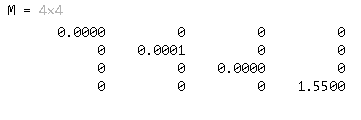
\includegraphics[width=.5\textwidth]{./assex/matrice_m.png}
\caption{matrice M}
\end{figure}
\begin{figure}[H]
\centering
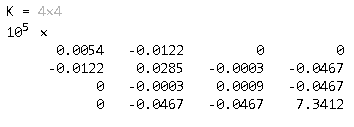
\includegraphics[width=.5\textwidth]{./assex/matrice_k.png}
\caption{matrice K}
\end{figure}
\begin{figure}[H]
\centering
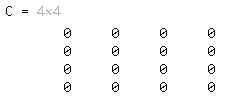
\includegraphics[width=.4\textwidth]{./assex/matrice_c.png}
\caption{matrice C}
\end{figure}
\begin{figure}[H]
\centering
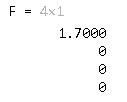
\includegraphics[width=.2\textwidth]{./assex/matrice_f.png}
\caption{vettore F}
\end{figure}
Abbiamo utilizzato una funzione chiamata show\_mode:
\begin{itemize}
    \item  che prende in input: M,K
    \item e fornisce in output: V,D
\end{itemize}
Dove V è una matrice che ha per colonna un gli autovettori che rappresentano i modi di vibrare nella cosiddetta analisi modale  e  D è una matrice diagonale di autovalori che contengono le pulsazioni naturali elevate al quadrato.
Prima dell'utilizzo della funzione c'è stato il problema della normalizzazione. In quanto posso normalizzare rispetto gli autovalori, la matrice delle masse oppure rispetto alla matrice k. La normalizzazione rispetto alla massa il legame di ortogonalità della matrice M e K, questo si traduce fisicamente nel dire che ciascuna forma modale è unica quindi nessun modo può essere ottenuto tramite combinazione di altri modi.La normalizzazione rispetto al massimo spostamento posto uguale a 1 è utile nella determinazione di diversi componenti a ciascun modo proprio di vibrare della struttura. Noi abbiamo optato per la seconda soluzione.
Il risultato ottenuto dalla funzione show\_mode:

\begin{figure}[H]
\centering
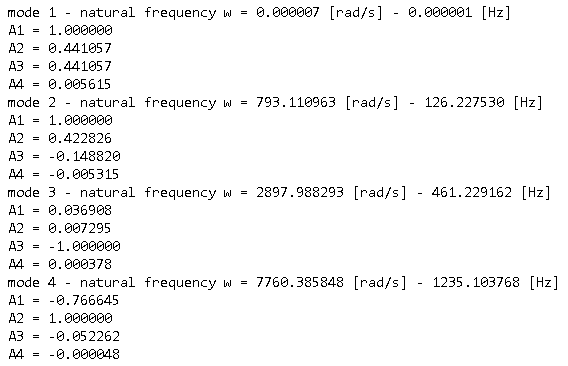
\includegraphics[width=.8\textwidth]{./assex/modi.png}
\caption{modi di vibrare, pulsazioni e frequenze}
\end{figure}
La normalizzazione per gli autovalori si può osservare dalla presenza di '1' in ogni modo di vibrare.Per quanto riguarda il primo modo di vibrare consideriamo la pulsazione e la frequenza entrambi uguali a 0.
\begin{figure}[H]
\centering
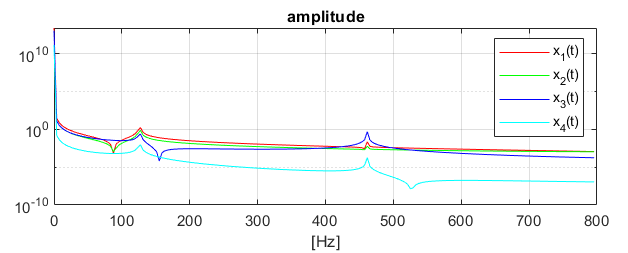
\includegraphics[width=.8\textwidth]{./assex/plot_c0.png}
\caption{ asse x: frequenze - asse y: ampiezze di vibrazione}
\end{figure}
Ora devo includere anche gli smorzamenti, quindi si fa l'ipotesi di uno smorzamento proporzionale. In questo modo vale la relazione:
\begin{equation*}
\phi' C \phi = A(M_{modale})+ B(K_{modale})= C_{modale}
\end{equation*}
Dove:
\begin{equation*}
c_i=2\xi \omega_i , i=j
\end{equation*}
\begin{equation*}
c_i=0 , i\neq j
\end{equation*}
Abbiamo ipotizzato un valore del coefficiente di smorzamento pari a 0.7. Per ottenere la matrice C dobbiamo calcolare le matrici $M_{modale}$ e $K_{modale}$ e $C_{modale}$
\begin{equation*}
\centering
    M_{mod} = \phi' M \phi
\end{equation*}
\begin{equation*}
\centering
    K_{mod} = \phi' k \phi
\end{equation*}
\begin{equation*}
\centering
    C_{mod} = 2 \xi \sqrt{M_{mod}K_{mod}}
\end{equation*}
Così posso ottenere:
\begin{equation*}
\centering
    C = \phi'^{-1} C_{mod} \phi^{-1}
\end{equation*}
\begin{figure}[H]
\centering
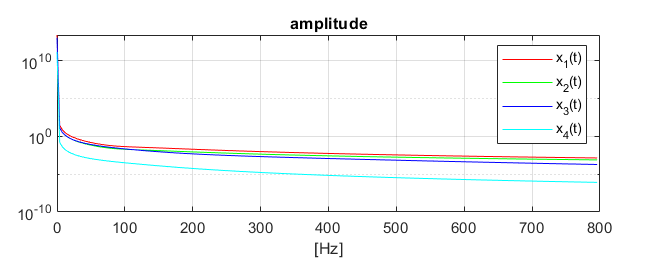
\includegraphics[width=.8\textwidth]{./assex/plot_c.png}
\caption{ asse x: frequenze - asse y: ampiezze di vibrazione}
\end{figure}
%-------------------------------- Simulazione modello asse y--------------------------------------------
\subsection{Simulazione modello Asse Y}
Si inizia con la inizializzazione dei dati illustrati nei sotto-capitoli precedenti. Le rigidezze specifiche sono state moltiplicate per $10^3 $ per avere $N/m$. Successivamente si inizia con il ricavare nuove informazione dai dati fornitoci. Per esempio il calcolo dei raggi delle pulegge e la lunghezza della cinghia tra puleggia-puleggia, carrello-puleggia e puleggia-carrello.
Per il calcolo della lunghezza dei tratti di cinghia ho utilizzato
la seguente espressione:

\begin{equation*}
L_{tot} = 2C +1.57(D+d) + \frac{(D+d)^2}{4C}
\end{equation*}
Per il tratto 1:
\begin{equation}
L_{1_{intermedio}} = L-\pi(R_1 + R_2)
\end{equation}
\begin{equation}
L_{1} = \frac{L_{1_{intermedio}}}{2} = 121.9 [mm]
\end{equation}
Per il tratto 2:
\begin{equation}
L_{2_{intermedio}} = L-(2\pi R_3)
\end{equation}
\begin{equation}
L_{2} = \frac{L_{2_{intermedio}}}{2} = 103.6 [mm]
\end{equation}
Adesso conoscendo la lunghezza dei vari tratti e le rigidezze specifiche delle varie cinghie posso calcolare le rigidezze $k_{1},k_{2},k_{3}$ e $k_{4}$:

\begin{equation*}
k_{1} = k_{cs_1}\frac{W_1}{L_1}
\end{equation*}
\begin{equation*}
k_{2} = k_{3} = k_{cs_2}\frac{2W_2}{L_2}
\end{equation*}
\begin{equation*}
k_{4} = k_{cs_2}\frac{W_2}{L_2}
\end{equation*}
Nella fase iniziale abbiamo considerato gli smorzamento uguali a zero, quindi:
\begin{equation*}
c_{1} = c_{2} = c_{3} = c_{4} = 0
\end{equation*}
Ora posso ricostruire le matrici definite del modello definite nel capitolo precedente:
\begin{figure}[H]
\centering
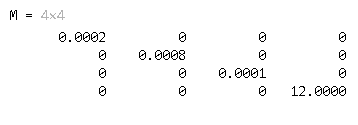
\includegraphics[width=.5\textwidth]{./assey/matrice_m.png}
\caption{matrice M}
\end{figure}
\begin{figure}[H]
\centering
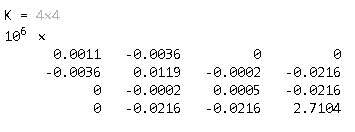
\includegraphics[width=.5\textwidth]{./assey/matrice_k.png}
\caption{matrice K}
\end{figure}
\begin{figure}[H]
\centering
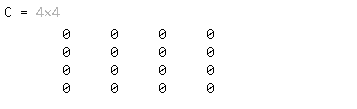
\includegraphics[width=.5\textwidth]{./assey/matrice_c.png}
\caption{matrice C}
\end{figure}
\begin{figure}[H]
\centering
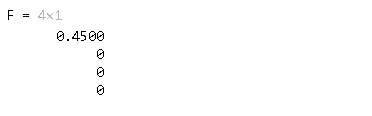
\includegraphics[width=.5\textwidth]{./assey/vettore_f.png}
\caption{vettore F}
\end{figure}
Abbiamo utilizzato anche qua la funzione chiamata show\_mode:

\begin{figure}[H]
\centering
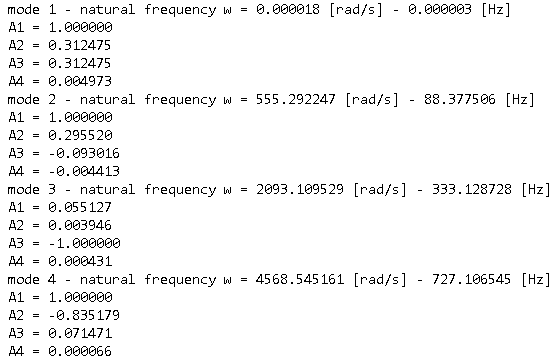
\includegraphics[width=.8\textwidth]{./assey/modi.png}
\caption{modi di vibrare, pulsazioni e frequenze}
\end{figure}
La normalizzazione per gli autovalori si può osservare dalla presenza di '1' in ogn modo di vibrare.Per quanto riguarda il primo modo di vibrare consideriamo la pulsazione e la frequenza entrambi uguali a 0.
\begin{figure}[H]
\centering
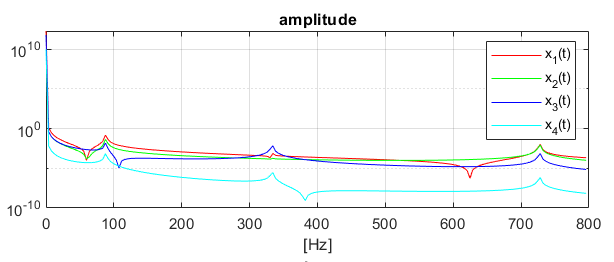
\includegraphics[width=.8\textwidth]{./assey/plot_c0.png}
\caption{ asse x: frequenze - asse y: ampiezze di vibrazione}
\end{figure}
Applico le stesse ipotesi fatte per l'asse x per ottenre la matrice C:
\begin{figure}[H]
\centering
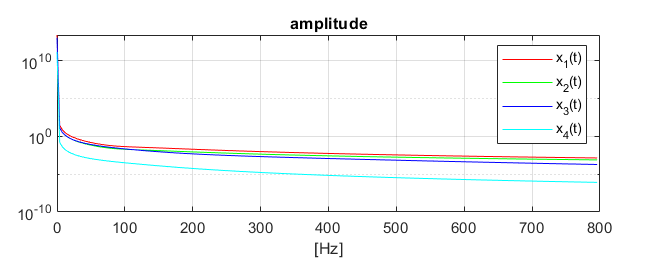
\includegraphics[width=.8\textwidth]{./assex/plot_c.png}
\caption{ asse x: frequenze - asse y: ampiezze di vibrazione}
\end{figure}


\section{Modellizzazione ASSE Y 5gdl}
In questo caso devo considerare che tra la puleggia $\theta_2$ e $\theta_3$ sono presenti le componenti torsionali. In questo caso la devo considerare 2 volte in quanto $\theta_2$ sta tra 2 pulegge caratterizzate dalla variabile $\theta_3$.
\subsection{Tratto 1}
$T = T_{puleggia_1} + T_{puleggia_2}+ T_{motore}
= {1 \over 2}J_{p_1}\dot{\theta_{1}}^{2}+ {1 \over 2}J_{p_2}\dot{\theta_{2}}^{2} + {1 \over 2}J_{m}\dot{\theta_{1}}^{2}$
\\
\\
$U = U_{gravitazionale} + U_{cinghie}
=  2[ {1 \over 2}k _{1}(\theta_{2}R_{2}-\theta_{1}R_{1})^{2} ]$
\\
\\
$D = 2[ {1 \over 2}c _{1}(\dot{\theta_{2}} R_{2}-\dot{\theta_{1}}R_{1})^{2} ]$
\\
\\
%                                            INIZIO EQUAZIONI DI LAGRANDE PER LA COORDINATA THETA1 
Coordinata libera $\theta_{1}$:
\\
\\

\begin{equation*}
{ \partial T \over \partial \theta_{1}} = 0 ; { \partial T \over \partial   \dot{\theta_{1}} } = 0;  \frac{d}{dT}(\frac{\partial T}{\partial \dot{\theta_{1}}})  = \ddot{\theta_{1}}(J_{p1} + J_{m})
\end{equation*}
\begin{equation*}
\frac{\partial U}{\partial \theta_{1}} = -2k_{1}R_{1}(\theta_{2}R_{2} - \theta_{1}R_{1});
\frac{\partial D}{\partial \dot{\theta_{1}}} = -2c_{1}R_{1}(\dot{(\theta_{2}}R_{2} - \dot{(\theta_{1}}R_{1})
\end{equation*}
\\
% PRIMA EQUAZIONE DEL TRATTO 1
Da cui ottengo la prima equazione: 
\\
\begin{equation*}
 \ddot{\theta_{1}}(J_{p1}+J_{m}) - R_{1}[2k_{1}(\theta_{2}R_{2}-\theta_{1}R_{1})+ 2c_{1}(\dot{\theta_{2}}R_{2}-\dot{\theta_{1}}R_{1})] = Q_{\theta_1}
\end{equation*}
\\
%                                           INIZIO EQUAZIONI DI LAGRANDE PER LA COORDINATA THETA2 
Coordinata libera $\theta_{2}$:
\\
\\
\begin{equation*}
{ \partial T \over \partial \theta_{2}} = 0 ; { \partial T \over \partial   \dot{\theta_{2}} } = \dot{\theta_{2}}J_{p2};  \frac{d}{dT}(\frac{\partial T}{\partial \dot{\theta_{2}}})  = \ddot{\theta_{2}}J_{p2}
\end{equation*}

\begin{equation*}
\frac{\partial U}{\partial \theta_{2}} = 2k_{1}R_{2}(\theta_{2}R_{2} - \theta_{1}R_{1})
\frac{\partial D}{\partial \dot{\theta_{2}}} = 2c_{1}R_{2}(\dot{\theta_{2}}R_{2} - \dot{\theta_{1}}R_{1})
\end{equation*}
\\
%                                            SECONDA EQUAZIONE DEL TRATTO 1
Da cui ottengo la seconda equazione: 
\\
\begin{equation*}
 \ddot{\theta_{2}}(J_{p2}) + R_{2}[2k_{1}(\theta_{2}R_{2}-\theta_{1}R_{1})+ 2c_{1}(\dot{\theta_{2}}R_{2}-\dot{\theta_{1}}R_{1})] = Q_{\theta_2}
\end{equation*}
\\
%---------------------------------------------------- EQUAZIONI DEL TRATTO 1-----------------------------------------------------------------------
ricapitolando ottengo un sistema di due equazioni:
\begin{equation*}
\begin{cases}
\ddot{\theta_{1}}(J_{p1}+J_{m}) - R_{1}[2k_{1}(\theta_{2}R_{2}-\theta_{1}R_{1})+ 2c_{1}(\dot{\theta_{2}}R_{2}-\dot{\theta_{1}}R_{1})] = Q_{\theta_1}\\

\ddot{\theta_{2}}(J_{p2}) + R_{2}[2k_{1}(\theta_{2}R_{2}-\theta_{1}R_{1})+ 2c_{1}(\dot{\theta_{2}}R_{2}-\dot{\theta_{1}}R_{1})] = Q_{\theta_2}
\end{cases}
\end{equation*}
%---------------------------------------------------- FINE EQUAZIONI DEL TRATTO 1-----------------------------------------------------------------------

\subsection{Tratto 2}

$T = T_{asse_x} + T_{puleggia_2}+ T_{puleggia_3} + T_{puleggia_3} + J_{albero}
=  J_{p_3}\dot{\theta_{4}}^{2}  + J_{p_3}\dot{\theta_{3}}^{2}+ \frac{1}{2}J_{p_2}\dot{\theta_{2}}^{2}+ {1 \over 2}m\dot{x}^{2} +J_{s}\dot{\theta_{2}}^{2} $
\\
\\
$U = U_{gravitazionale} + U_{cinghie} + U_{albero} $
\\
$ = k_{4}(x)(\theta_{3}R_{3}-\theta_{4}R_{3})^{2} +k_{3}(x)(x-\theta_{4}R_{3})^{2}+k_{2}(x)(x-\theta_{3}R_{3})^{2}+ k_{T}(\theta_{3}-\theta{2})^{2}$
\\
\\
$D  = c_{4}(x)(\dot{\theta_{3}}R_{3}-\dot{\theta_{4}}R_{3})^{2} +c_{3}(x)(\dot{x}-\dot{\theta_{4}}R_{3})^{2}+c_{2}(x)(\dot{x}-\dot{\theta_{3}}R_{3})^{2}+ c_{T}(\dot{\theta_{3}}-\dot{\theta{2}})^{2}$
\\
\\
Nota: 
$$c_{2}(x), c_{3}(x),k_{2}(x), k_{3}(x)$$ sono variabili.
\\
\\
Notazione:
\begin{equation*}
c_{2}(x) = c_{2};
c_{3}(x) = c_{3};
k_{2}(x) = k_{2};
k_{3}(x) = k_{3};
\end{equation*}
\\
%                                            INIZIO EQUAZIONI DI LAGRANDE PER LA COORDINATA X 
Coordinata libera $x$:
\\
\\
\begin{equation*}
\frac{ \partial T}{\partial x} = 0 ; \frac{\partial T}{\partial \dot{x}} = \dot{x}m;  \frac{d}{dT}(\frac{\partial T}{\partial \dot{x}})  = \ddot{x}m;
\end{equation*}
\\
\\
\begin{equation*}
\frac{\partial U}{\partial x} = 2k_3(x-\theta_4R_3) + 2k_2(x -\theta_3R_3)
\end{equation*}
\\
\\
\begin{equation*}
\frac{\partial D}{\partial \dot{x}} = 2c_3(\dot{x}-\dot{\theta_4}R_3) + 2c_2(\dot{x} -\dot{\theta_3}R_3)
\end{equation*}
\\
% PRIMA EQUAZIONE DEL TRATTO 2
Da cui ottengo la prima equazione: 
\\
\begin{equation*}
 \ddot{x}m + 2k_{3}(x-\theta_{4}R_{3}) + 2k_{2}(x- \theta_{3}R_{3})+ 2c_{3}(\dot{x}-\dot{\theta_4}R_{3}) + 2c_{2}(\dot{x} - \dot{\theta_{3}}R_{3}) = Q_x
\end{equation*}
\\
%                                            INIZIO EQUAZIONI DI LAGRANGE PER LA COORDINATA THETA2 
Coordinata libera $\theta_2$:
\\
\\
\begin{equation*}
\frac{ \partial T}{\partial \theta_2} = 0 ; \frac{\partial T}{\partial \dot{\theta_2}} = \dot{\theta_2}J_{p_2}+ 2\dot{\theta_2}J_{s};  \frac{d}{dT}(\frac{\partial T}{\partial \dot{\theta_2}})  = \ddot{\theta_2}J_{p_3}+2\ddot{\theta_2}J_{s}
\end{equation*}
\\
\\
\begin{equation*}
\frac{\partial U}{\partial \theta_2} = -2k_T(\theta_3-\theta_2) 
\end{equation*}
\\
\\
\begin{equation*}
\frac{\partial D}{\partial \dot{\theta_2}} =  -2c_T(\dot{\theta_3}-\dot{\theta_2})
\end{equation*}
\\
% SECONDA EQUAZIONE DEL TRATTO 2
Da cui ottengo la seconda equazione: 
\\
\begin{equation*}
 \ddot{\theta_2}(J_{p_2} + 2 J_s) - 2k_{T}(\theta_{3} - \theta_{2}) + 2c_{T}(\dot{\theta_{3}} - \dot{\theta_{2}})= Q_{\theta_2}
\end{equation*}
%                                            INIZIO EQUAZIONI DI LAGRANDE PER LA COORDINATA THETA3
Coordinata libera $\theta_3$:
\\
\\
\begin{equation*}
\frac{ \partial T}{\partial \theta_3} = 0 ; \frac{\partial T}{\partial \dot{\theta_3}} = 2J_{p_3}\dot{\theta_3};  \frac{d}{dT}(\frac{\partial T}{\partial \dot{\theta_3}})  = 2\ddot{\theta_3}J_{p_3}
\end{equation*}
\\
\\
\begin{equation*}
\frac{\partial U}{\partial \theta_3} = -2k_2R_3(x - \theta_3R_3) + 2k_4R_3(\theta_3 R_3 - \theta_4 R_3) + 2k_T(\theta_3 -  \theta_2)
\end{equation*}
\\
\\
\begin{equation*}
\frac{\partial D}{\partial \dot{x}} =  -2c_2R_3(\dot{x} - \dot{\theta_3}R_3) + 2c_4R_3(\dot{\theta_3} R_3 - \dot{\theta_4} R_3) +
2c_T(\dot{\theta_3} - \dot{ \theta_2})
\end{equation*}
\\
% TERZA EQUAZIONE DEL TRATTO 2
Da cui ottengo la terza equazione: 
\\
\begin{equation*}
 2\ddot{\theta_3}J_{p_3}+  2k_T(\theta_3 -  \theta_2) + 2c_T(\dot{\theta_3} - \dot{ \theta_2}) -2k_2R_3(x - \theta_3R_3) + 
\end{equation*}
\begin{equation*}
     2k_4R_3(\theta_3 R_3 - \theta_4 R_3)  -2c_2R_3(\dot{x} - \dot{\theta_3}R_3) +  2c_4R_3(\dot{\theta_3} R_3 - \dot{\theta_4} R_3) = Q_{\theta_3}
\end{equation*}
\\
%-------------- INIZIO EQUAZIONI DI LAGRANGE PER LA COORDINATA THETA 4
Coordinata libera $\theta_4$:
\\
\\
\begin{equation*}
\frac{ \partial T}{\partial \theta_4} = 0 ; \frac{\partial T}{\partial \dot{\theta_4}} = 2J_{p_3}\dot{\theta_4};  \frac{d}{dT}(\frac{\partial T}{\partial \dot{\theta_4}})  = 2\ddot{\theta_4}J_{p_3}
\end{equation*}
\\
\\
\begin{equation*}
\frac{\partial U}{\partial \theta_3} = -2k_3R_3(x - \theta_4R_3) - 2k_4R_3(\theta_3 R_3 - \theta_4 R_3) 
\end{equation*}
\\
\\
\begin{equation*}
\frac{\partial D}{\partial \dot{x}} =  -2c_3R_3(\dot{x} - \dot{\theta_4}R_3) - 2c_4R_3(\dot{\theta_3} R_3 - \dot{\theta_4} R_3)
\end{equation*}
\\
% QUARTA EQUAZIONE DEL TRATTO 2
Da cui ottengo la quarta equazione: 
\\
\begin{equation*}
 2\ddot{\theta_4}J_{p_3} -2k_3R_3(x - \theta_4R_3) - 2k_4R_3(\theta_3 R_3 - \theta_4 R_3) +
\end{equation*}
\begin{equation*}
-2c_3R_3(\dot{x} - \dot{\theta_4}R_3) - 2c_4R_3(\dot{\theta_3} R_3 - \dot{\theta_4} R_3)
      = Q_{\theta_4}
\end{equation*}
%---------------------------------------------------- EQUAZIONI DEL TRATTO 2-----------------------------------------------------------------------
ricapitolando ottengo un sistema di cinque equazioni:
\begin{equation*}
\begin{cases}

 \ddot{x}m + 2k_{3}(x-\theta_{4}R_{3}) + 2k_{2}(x- \theta_{3}R_{3})+ 2c_{3}(\dot{x}-\dot{\theta_4}R_{3}) + 2c_{2}(\dot{x} - \dot{\theta_{3}}R_{3}) = 0\\
 
 \ddot{\theta_{1}}(J_{p1}+J_{m}) - R_{1}[2k_{1}(\theta_{2}R_{2}-\theta_{1}R_{1})+ 2c_{1}(\dot{\theta_{2}}R_{2}-\dot{\theta_{1}}R_{1})] = C_{m}\\
 
  \ddot{\theta_2}(J_{p_2} + 2 J_s) - 2k_{T}(\theta_{3} - \theta_{2}) - 2c_{T}(\dot{\theta_{3}} - \dot{\theta_{2}})+ R_{2}[2k_{1}(\theta_{2}R_{2}-\theta_{1}R_{1})+ 2c_{1}(\dot{\theta_{2}}R_{2}-\dot{\theta_{1}}R_{1})]= 0 \\
  
 \ddot{\theta_3}(2J_{p_3})+  2k_T(\theta_3 -  \theta_2) + 2c_T(\dot{\theta_3} - \dot{ \theta_2}) -2k_2R_3(x - \theta_3R_3) + \\
     2k_4R_3(\theta_3 R_3 - \theta_4 R_3)  -2c_2R_3(\dot{x} - \dot{\theta_3}R_3) +  2c_4R_3(\dot{\theta_3} R_3 - \dot{\theta_4} R_3) = 0\\
     
 \ddot{\theta_4}(2J_{p_3}) -2k_3R_3(x - \theta_4R_3) - 2k_4R_3(\theta_3 R_3 - \theta_4 R_3) +\\
-2c_3R_3(\dot{x} - \dot{\theta_4}R_3) - 2c_4R_3(\dot{\theta_3} R_3 - \dot{\theta_4} R_3)
      = 0
\end{cases}
\end{equation*}

Definisco le matrici M,K,C ed F per esprimere tutto in notazione matriciale:
\\
\\
M= 
$$
\begin{bmatrix}
m & 0 & 0 & 0 & 0\\ 
0 & J_{p_1}+J_m & 0 & 0 & 0\\
0 & o & J_{p_2}+2J_{s} & 0 & 0\\
0 & 0 & 0 & 2J_{p_3} & 0\\
0 & 0 & 0 &  0 & 2J_{3}
\end{bmatrix}
$$
K= 
$$
\begin{bmatrix}

2k_1R_{1}^2 & -2k_{1}R_{2}R{1} & 0 & 0 & 0\\
-2k_1R_{1}R_{2} & 2k_{T} + 2k_{1}R_{2}^2 & -2k_{T} & 0 & 0\\
0 & -2k_{T} & 2k_{T} + k_{2}R_{3}^2 + k_{4}R_{3}^2 & - 2R_{3}^2k_{4} & -2k_{2}R_{3}\\
0 & 0 & -2R_{3}^2k_{4} & 2R_{3}^2k_{3} + 2R_{3}^2k_{4} & -2R_{3}k_{3} \\
0 & 0 &  -2k_{2}R_{3} & -2R_{3}k_{3} & 2k_2 + 2k_3\\
\end{bmatrix}
$$
C= 
$$
\begin{bmatrix}
2c_1R_{1}^2 & -2c_{1}R_{2}R{1} & 0 & 0 & 0\\
-2c_1R_{1}R_{2} & 2c_{T} + 2c_{1}R_{2}^2 & -2c_{T} & 0 & 0\\
0 & -2c_{T} & 2c_{T} + c_{2}R_{3}^2 + c_{4}R_{3}^2 & - 2R_{3}^2c_{4} & -2c_{2}R_{3}\\
0 & 0 & -2R_{3}^2c_{4} & 2R_{3}^2c_{3} + 2R_{3}^2c_{4} & -2R_{3}c_{3} \\
0 & 0 &  -2c_{2}R_{3} & -2R_{3}c_{3} & 2c_2 + 2c_3\\
\end{bmatrix}
$$
F= 
$$
\begin{bmatrix}
C_m \\
0 \\
0\\
0\\
0
\end{bmatrix}
$$
ottengo così la relazione matriciale:


$$ M\ddot{X} + C\dot{X} + KX = F $$
dove:
\\
\\
X= 
$$
\begin{bmatrix}

\theta_1 \\
\theta_2\\
\theta_3\\
\theta_4\\
x 
\end{bmatrix}
$$
$\dot{X}$= 
$$
\begin{bmatrix}
\dot{\theta_1} \\
\dot{\theta_2}\\
\dot{\theta_3}\\
\dot{\theta_4}\\
\dot{x} 
\end{bmatrix}
$$
$\ddot{X}$= 
$$
\begin{bmatrix}
\ddot{\theta_1} \\
\ddot{\theta_2}\\
\ddot{\theta_3}\\
\ddot{\theta_4}\\
\ddot{x} 
\end{bmatrix}
$$

Utilizzando questo modello possiamo notare un modo di vibrare molto alto rispetto agli altri. Questo per l'analisi che vogliamo fare può essere trascurato e abbiamo deciso di utilizzare un modello a 4 GDL, che ci permette di semplificare il sistema, ritenendo trascurabile la deformazione torsionale dell'albero.
Come si può vedere, questa approssimazione non porta una significativa variazione nei primi quattro moduli di vibrare e il modello sebra rappresentare in modo corretto la situazione.
\begin{figure}[H]
\centering
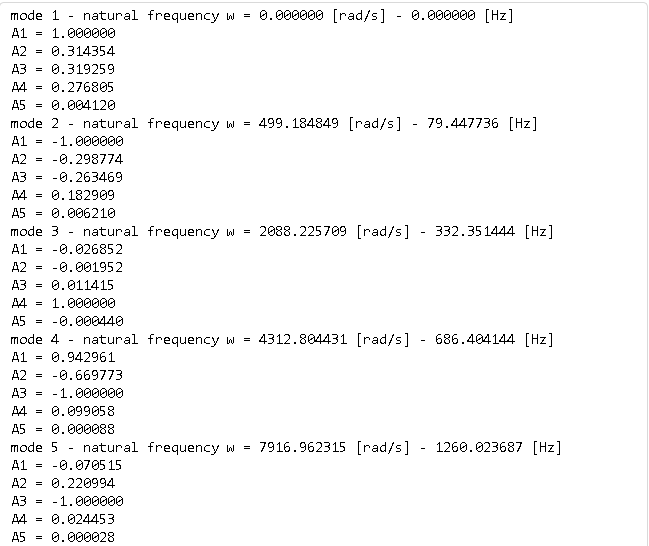
\includegraphics[width=.8\textwidth]{./assey/modi5.png}
\end{figure}
\begin{figure}[H]
\centering
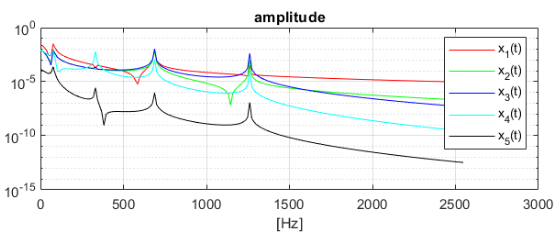
\includegraphics[width=.8\textwidth]{./assey/ampiezzamodi5.png}
\end{figure}

\section{Struttura del codice}
Abbiamo suddiviso il codice principale in più parti, per facilitare la gestione del progetto. In particolare, abbiamo creato due strutture con le informazione degli assi x e y (parx e pary). Un file chiamato "m" con le informazioni per la configurazione dei motori e infine 4 funzioni utilizzate per rappresentare i controllori:
\begin{itemize}
    \item ac = anello di corrente
    \item av = anello di velocità
    \item ap = anello di posizione
    \item pp = posizionameto poli
\end{itemize}

\section{Simulazione modello su Simulink}

\subsection{Asse x}

Le equazioni differenziali del modello scritte in matlab nel capitolo precedente le rappresento in questo modo in Simulink:
\begin{figure}[H]
\centering
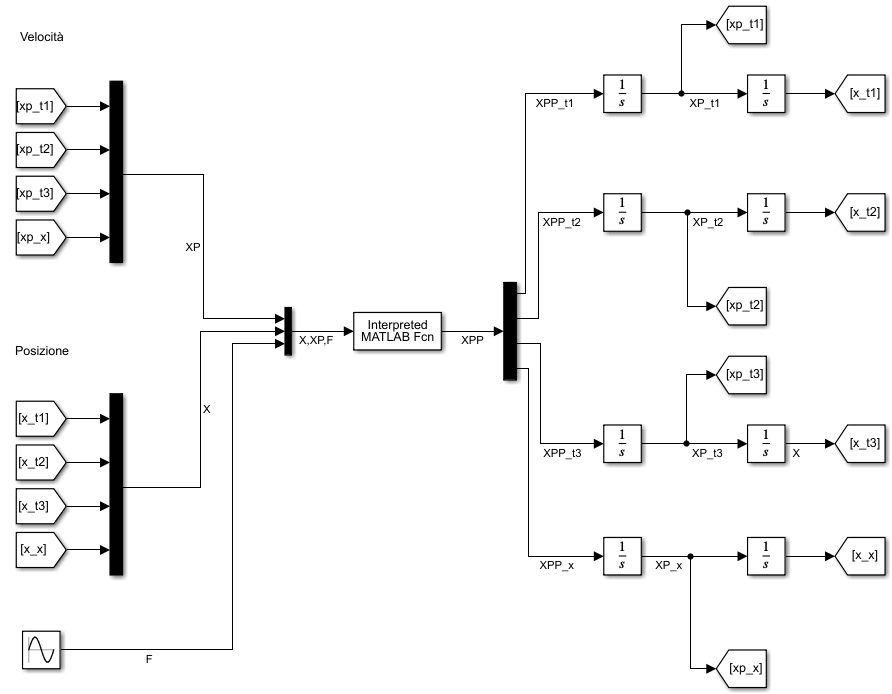
\includegraphics[width=.8\textwidth]{./simulink/assex/modellox.png}
\caption{ Simulink modello x}
\end{figure}
Si osserva che nel Simulink è presente una Matlab Function contenente la funzione Accelerazioni() . Questa ha il compito di calcolare le derivate seconde al tempo $t$ e partendo da questo possiamo andare ad integrare per calcolare velocità e posizioni al tempo $t+1$.
Nel caso in cui si considerino rigidezze e smorzamenti variabili nel tempo, la funzione si occupa di tenere conto dello spostamento del carrello per aggiornare i valori istante per istante in funzione della lunghezza del tratto di cinghia.
\subsection{Verifica del modello dell'asse x}



\subsection{Asse y}
Anche per l'asse y possiamo procedere in modo analogo:
\begin{figure}[H]
\centering
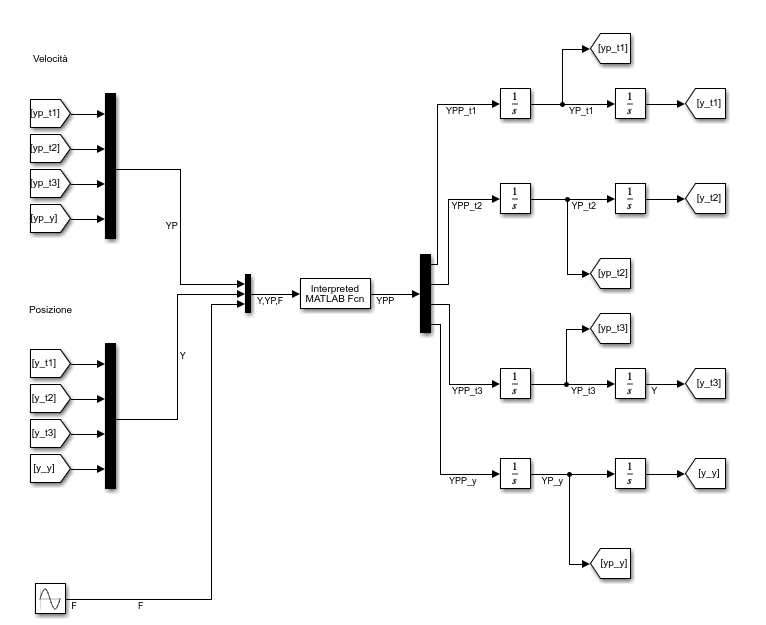
\includegraphics[width=.8\textwidth]{./simulink/assey/modelloy.png}
\caption{ Simulink modello y}
\end{figure}
\section{Test di verifica del modello su asse X,Y}

\subsection{Test per i modi di vibrare}
Verifica fatta con la matrice K costante, ovvero con rigidezze costanti.Questo test serve per verificare che il modello sia stato scritto correttamente
e che risponda come previsto:
il sistema è lineare e applicando una forzante, dobbiamo ottenere una risposta con la stessa frequenza della forzante.
Sempre con la matrice delle rigidezze costante, si può verificare che fissando come condizioni iniziali uno dei modi calcolati, il sistema si mette in vibrazione secondo quel modo.
Questo perché viene mantenuto il rapporto fra le ampiezze e le frequenze caratteristiche di quel modo di vibrare.

%La matrice di smorzamento in coordinate fisiche non viene ricalcolata %in modo corretto, ma viene ricalcolato in modo tale per cui dopo se %si fa la prova di assegnare condizioni iniziale
%il comportamento è tale per cui non torna.
%Ad esempio non torna sulla posizione di equilibrio iniziale, cosa che %non può accadere.
Metto a 0 anche la matrice degli smorzamenti per apprezzare ancora di più il risultato.
\subsection{Test sull'asse x}
\subsubsection{i=4 quarto modo di vibrare}
Trovo una frequenza di 1.292 Khz  , molto vicini ai 1235 Hz del  quarto modo di vibrare

\begin{figure}[H]
\centering
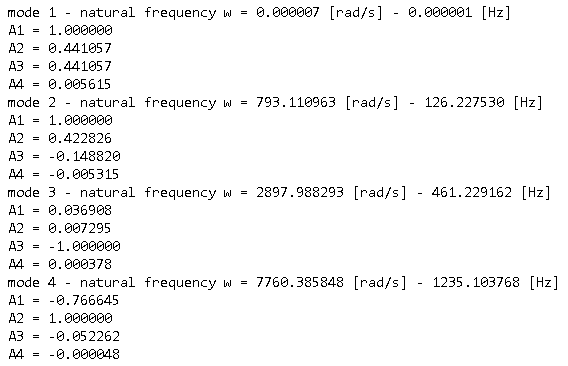
\includegraphics[width=.8\textwidth]{./assex/modi.png}
\caption{modi di vibrare, pulsazioni e frequenze assex}
\end{figure}

Ampiezze:
\begin{itemize}

    \item $x_{t_1}$ ha ampiezza pari a 1.46
    \begin{equation*}
    \frac{x_{t_1}}{x_{t_2}} = 0.76614338
    \end{equation*}
    
    \item $x_{t_2}$ ha ampiezza pari a 1.911
        \begin{equation*}
    \frac{x_{t_2}}{x_{t_2}} =  1
    \end{equation*}
    
    \item $x_{t_3}$ ha ampiezza pari a $9.985*10^{-2}$
        \begin{equation*}
    \frac{x_{t_3}}{x_{t_2}} = 0.05227
    \end{equation*}
    
    \item $	x_{x}$ ha ampiezza pari a $9.136*10^{-5}$
    \begin{equation*}
    \frac{x_{x}}{x_{t_2}} =  0.000047832
    \end{equation*}
    \end{itemize}
    
    
Risultati delle simulazioni con queste condizioni iniziali: 
\begin{enumerate}

    \item 
        Nota bene: Più le due misure sono vicine più la frequenza aumenta. Quindi posso considerare la frequenza tra due picchi la meta circa di quella illustrata nella tabella. Andamento della variabile $x_{t1}$:
        \begin{figure}[H]
        \centering
        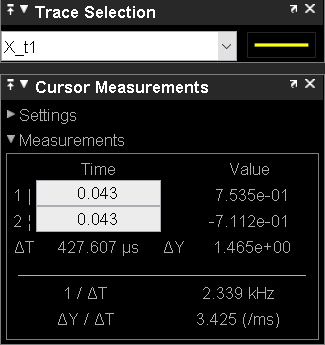
\includegraphics[width=7cm,height=7cm,keepaspectratio]{./simulink/assex/modo4_t1tab.png}
        \caption{Misure prese tra un picco ed il punto medio con il picco successivo}
        \end{figure}
        
        \begin{figure}[H]
        \centering
        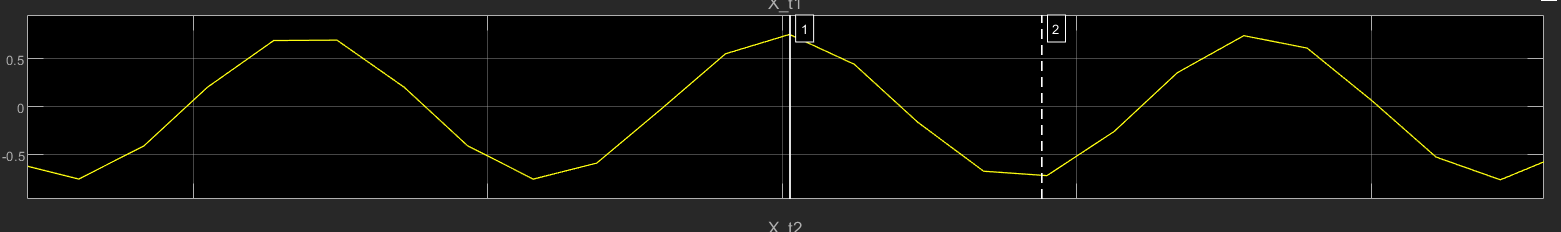
\includegraphics[width=12cm,height=10cm,keepaspectratio]{./simulink/assex/modo4_t1.png}
        \caption{andamento $x_{t1}$ con condizione iniziale il quarto modo di vibrare}
        \end{figure}

    \item
            Andamento della variabile $x_{t2}$:
    
\begin{figure}[H]
\centering
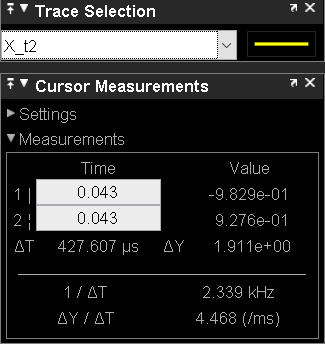
\includegraphics[width=7cm,height=7cm,keepaspectratio]{./simulink/assex/modo4_t2tab.png}
\caption{Misure prese tra un picco ed il punto medio con il picco successivo}
\end{figure}

\begin{figure}[H]
\centering
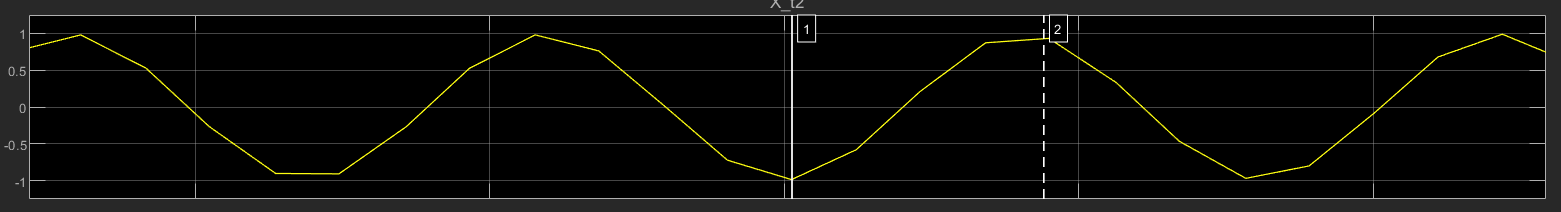
\includegraphics[width=12cm,height=10cm,keepaspectratio]{./simulink/assex/modo4_t2.png}
\caption{andamento $x_{t2}$ con condizione iniziale il quarto modo di vibrare}
\end{figure}
      
    \item 
       Andamento della variabile $x_{t3}$:

\begin{figure}[H]
\centering
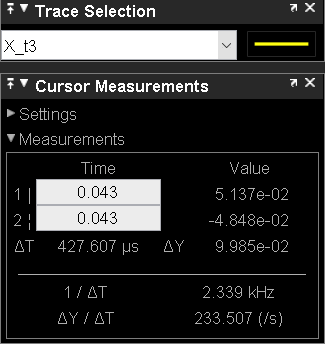
\includegraphics[width=7cm,height=7cm,keepaspectratio]{./simulink/assex/modo4_t3tab.png}
\caption{Misure prese tra un picco ed il punto medio con il picco successivo}
\end{figure}

\begin{figure}[H]
\centering
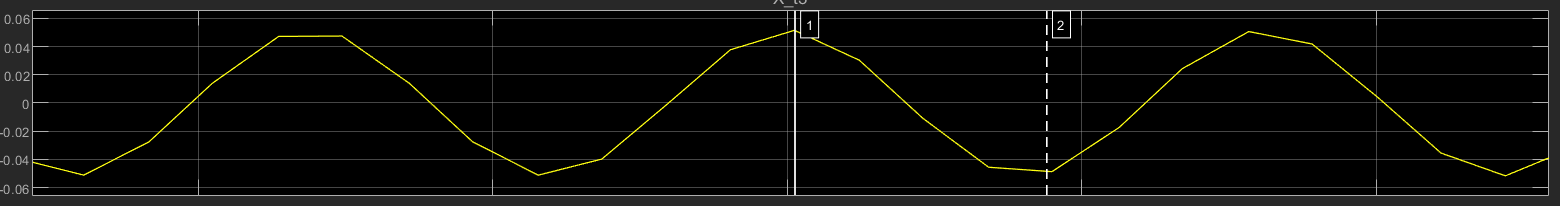
\includegraphics[width=12cm,height=10cm,keepaspectratio]{./simulink/assex/modo4_t3.png}
\caption{andamento $x_{t3}$ con condizione iniziale il quarto modo di vibrare}
\end{figure}

\item     
   Andamento della variabile $x_{x}$:
        
\begin{figure}[H]
\centering
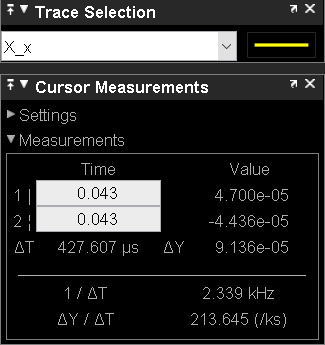
\includegraphics[width=7cm,height=7cm,keepaspectratio]{./simulink/assex/modo4_xtab.png}
\caption{Misure prese tra un picco ed il punto medio con il picco successivo}
\end{figure}
\begin{figure}[H]
\centering
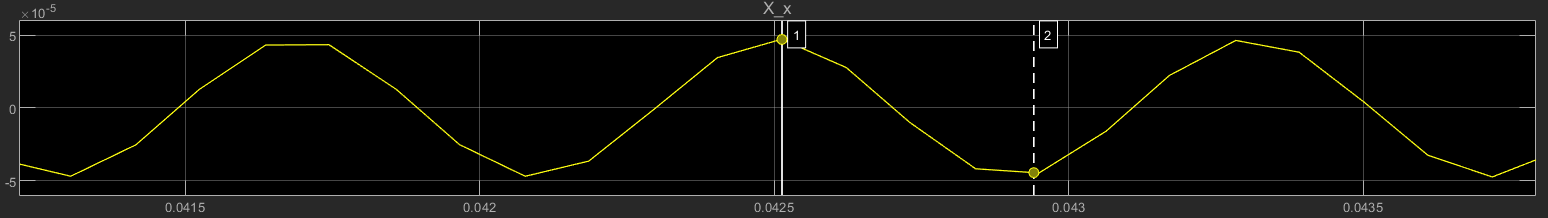
\includegraphics[width=12cm,height=10cm,keepaspectratio]{./simulink/assex/modo4_x.png}
\caption{andamento $x_{x}$ con condizione iniziale il quarto modo di vibrare}

\end{figure}
\end{enumerate}

%------------------------------------- terzo modo di vibrare ------------------------------
\subsubsection{i=3 terzo modo di vibrare}

Ampiezze:
\begin{itemize}

    \item $x_{t_1}$ ha ampiezza pari a $7.157*10^{-2}$
    \begin{equation*}
    \frac{x_{t_1}}{x_{t_3}} = 0.036910778
    \end{equation*}
    \begin{equation*}\frac{A1}{A3} = -0.036908 \end{equation*}
    
    \item $x_{t_2}$ ha ampiezza pari a $1.415*10^{-2}$
        \begin{equation*}
    \frac{x_{t_2}}{x_{t_3}} = 7.29757607*10^-3
    \end{equation*}
      \begin{equation*} \frac{A2}{A3} = -0.007295  \end{equation*}
    
    \item $x_{t_3}$ ha ampiezza pari a 1.939	
        \begin{equation*}
    \frac{x_{t_4}}{x_{t_3}} = 3.776173285*10^-4
    \end{equation*}
    \begin{equation*}  \frac{A4}{A3} = -0.000378 	 \end{equation*}
    
    \item $	x_{x}$ ha ampiezza pari a $7.322*10^{-4}$
    \end{itemize}
    
Risultati delle simulazioni con queste condizioni iniziali: 
\begin{enumerate}

    \item 
   Andamento della variabile $x_{t1}$:
       
        \begin{figure}[H]
        \centering
        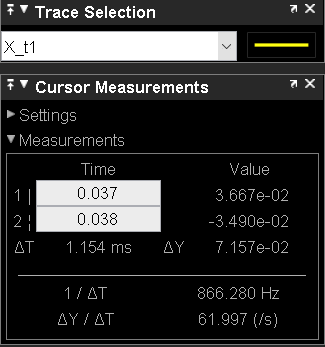
\includegraphics[width=7cm,height=7cm,keepaspectratio]{./simulink/assex/modo3_t1tab.png}
        \caption{Misure prese tra un picco ed il punto medio con il picco successivo}
        \end{figure}
        
        \begin{figure}[H]
        \centering
        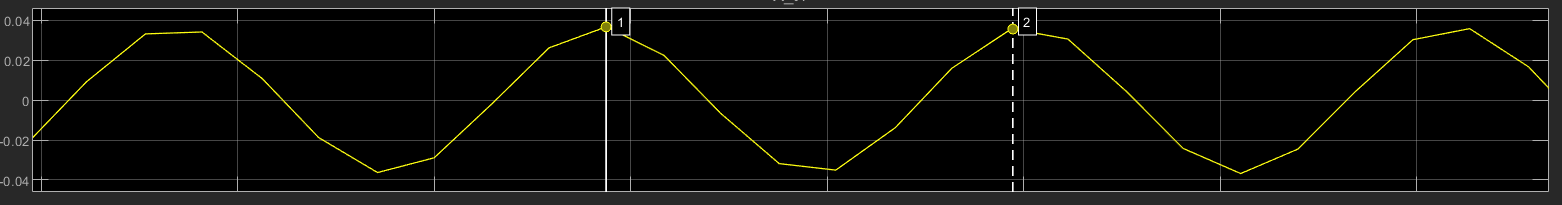
\includegraphics[width=12cm,height=10cm,keepaspectratio]{./simulink/assex/modo3_t1.png}
        \caption{andamento $x_{t1}$ con condizione iniziale il terzo modo di vibrare}
        \end{figure}

    \item
       Andamento della variabile $x_{t2}$:
\begin{figure}[H]
\centering
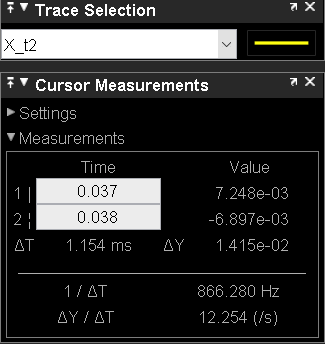
\includegraphics[width=7cm,height=7cm,keepaspectratio]{./simulink/assex/modo3_t2tab.png}
\caption{Misure prese tra un picco ed il punto medio con il picco successivo}
\end{figure}

\begin{figure}[H]
\centering
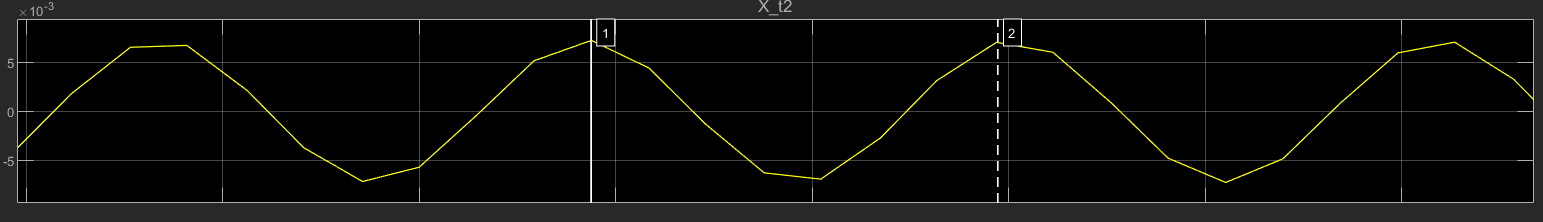
\includegraphics[width=12cm,height=10cm,keepaspectratio]{./simulink/assex/modo3_t2.png}
\caption{andamento $x_{t2}$ con condizione iniziale il terzo modo di vibrare}
\end{figure}
      
    \item 
Andamento della variabile $x_{t3}$:
\begin{figure}[H]
\centering
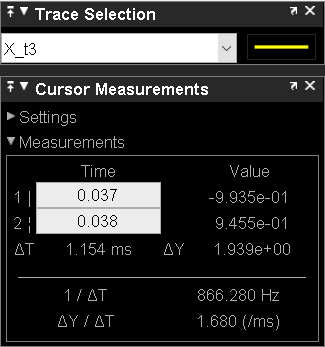
\includegraphics[width=7cm,height=7cm,keepaspectratio]{./simulink/assex/modo3_t3tab.png}
\caption{Misure prese tra un picco ed il punto medio con il picco successivo}
\end{figure}

\begin{figure}[H]
\centering
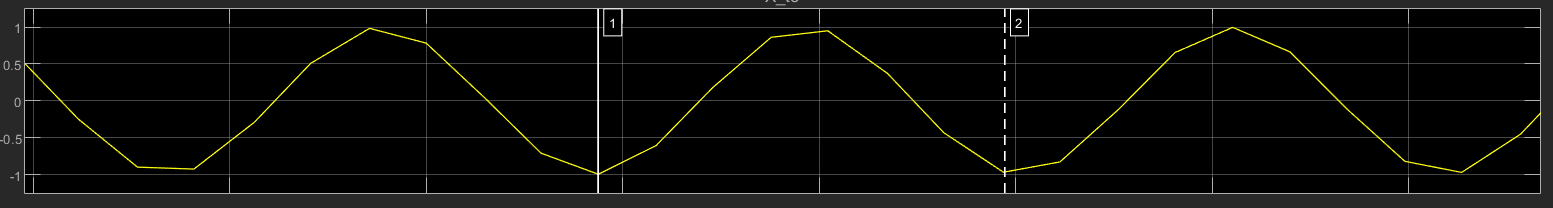
\includegraphics[width=12cm,height=10cm,keepaspectratio]{./simulink/assex/modo3_t3.png}
\caption{andamento $x_{t3}$ con condizione iniziale il terzo modo di vibrare}
\end{figure}


    \item
       Andamento della variabile $x_{x}$:
      
\begin{figure}[H]
\centering
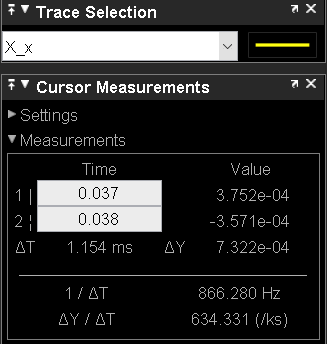
\includegraphics[width=7cm,height=7cm,keepaspectratio]{./simulink/assex/modo3_xtab.png}
\caption{Misure prese tra un picco ed il punto medio con il picco successivo}
\end{figure}

\begin{figure}[H]
\centering
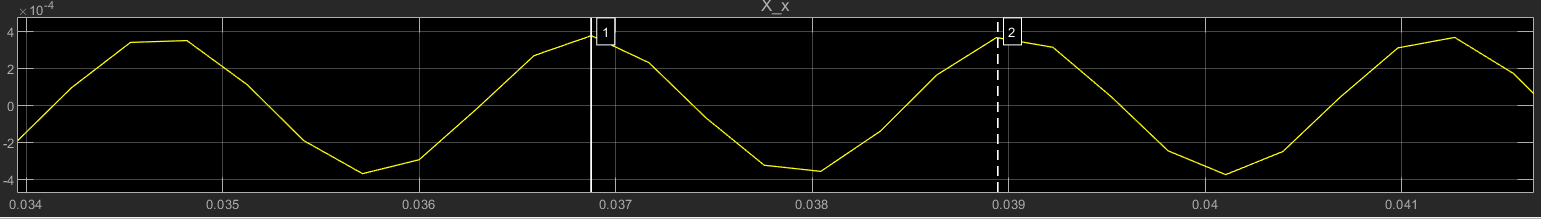
\includegraphics[width=12cm,height=10cm,keepaspectratio]{./simulink/assex/modo3_x.png}
\caption{andamento $x_{x}$ con condizione iniziale il terzo modo di vibrare}
\end{figure}
\end{enumerate}

%------------------------------------- secondo modo di vibrare ------------------------------
\subsubsection{i=2 secondo modo di vibrare}


Ampiezze:
\begin{itemize}

    \item $x_{t_1}$ ha ampiezza pari a $1.991$
    \begin{equation*} \frac{x_{t_2}}{x_{t_1}} = 0.4184329483 \end{equation*}
     \begin{equation*} 	\frac{A2}{A1} = 0.422826  \end{equation*}
    
    \item $x_{t_2}$ ha ampiezza pari a $ 8.331*10^{-1}$
        \begin{equation*} \frac{x_{t_3}}{x_{t_1}} = 0.1482672024 \end{equation*}
        \begin{equation*}  \frac{A3}{A1} = -0.148820 \end{equation*}
    
    \item $x_{t_3}$ ha ampiezza pari a $2.952*10^-1$
    \begin{equation*} \frac{x_{t_4}}{x_{t_1}} =  5.303867403*10^-3 \end{equation*}
    \begin{equation*}  \frac{A4}{A1} = -0.005315  	 \end{equation*}
    
    \item $	x_{x}$ ha ampiezza pari a $1.056*10^{-2}$
    \end{itemize}
    
Risultati delle simulazioni con queste condizioni iniziali: 
\begin{enumerate}

    \item 
     Andamento della variabile $x_{t1}$:
     
        \begin{figure}[H]
        \centering
        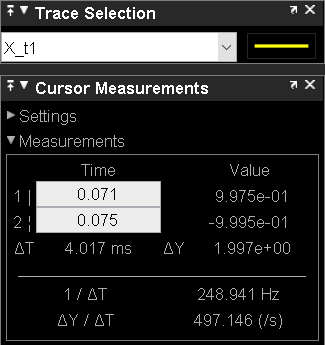
\includegraphics[width=7cm,height=7cm,keepaspectratio]{./simulink/assex/modo2_t1tab.png}
        \caption{Misure prese tra un picco ed il punto medio con il picco successivo}
        \end{figure}
        
        \begin{figure}[H]
        \centering
        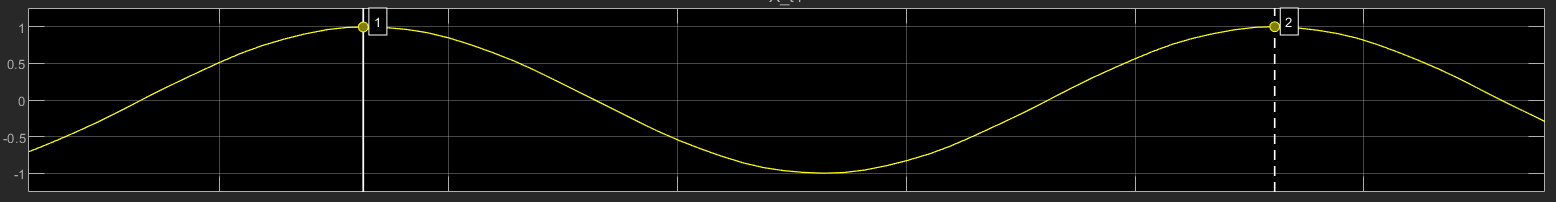
\includegraphics[width=12cm,height=10cm,keepaspectratio]{./simulink/assex/modo2_t1.png}
        \caption{andamento $x_{t1}$ con condizione iniziale il secondo modo di vibrare}
        \end{figure}

    \item
     Andamento della variabile $x_{t2}$:
\begin{figure}[H]
\centering
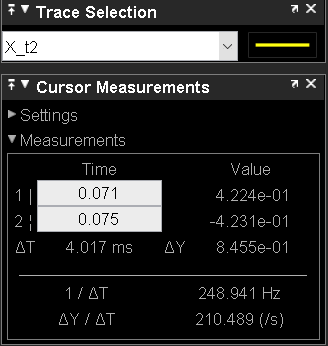
\includegraphics[width=7cm,height=7cm,keepaspectratio]{./simulink/assex/modo2_t2tab.png}
\caption{Misure prese tra un picco ed il punto medio con il picco successivo}
\end{figure}

\begin{figure}[H]
\centering
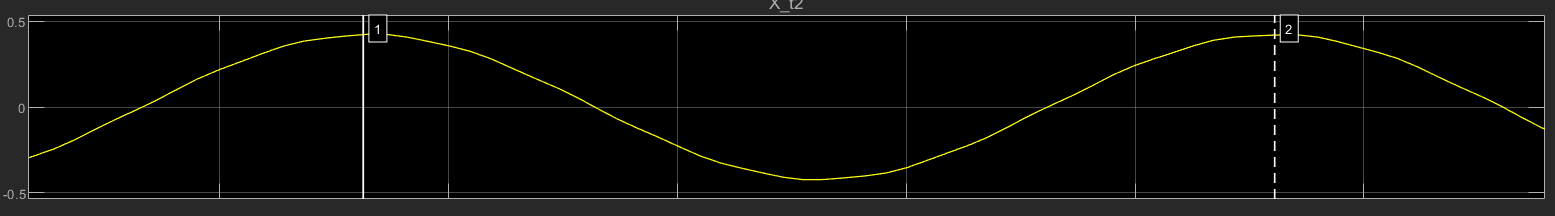
\includegraphics[width=12cm,height=10cm,keepaspectratio]{./simulink/assex/modo2_t2.png}
\caption{andamento $x_{t2}$ con condizione iniziale il secondo modo di vibrare}
\end{figure}
      
    \item 
Andamento della variabile $x_{t3}$:

\begin{figure}[H]
\centering
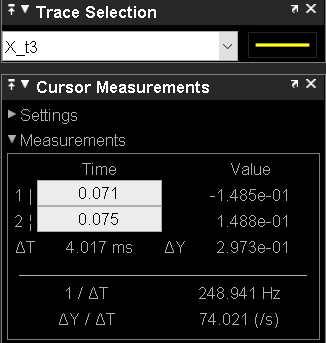
\includegraphics[width=7cm,height=7cm,keepaspectratio]{./simulink/assex/modo2_t3tab.png}
\caption{Misure prese tra un picco ed il punto medio con il picco successivo}
\end{figure}

\begin{figure}[H]
\centering
\includegraphics[width=12cm,height=10cm,keepaspectratio]{./simulink/assex/modo2_t3.png}
\caption{andamento $x_{t3}$ con condizione iniziale il secondo modo di vibrare}
\end{figure}

    \item
         Andamento della variabile $x_{x}$:
      
\begin{figure}[H]
\centering
\includegraphics[width=7cm,height=7cm,keepaspectratio]{./simulink/assex/modo2_xtab.png}
\caption{Misure prese tra un picco ed il punto medio con il picco successivo}
\end{figure}

\begin{figure}[H]
\centering
\includegraphics[width=12cm,height=10cm,keepaspectratio]{./simulink/assex/modo2_x.png}
\caption{andamento $x_{x}$ con condizione iniziale il secondo modo di vibrare}
\end{figure}
\end{enumerate}

%------------------------------------- primo modo di vibrare ------------------------------
\subsubsection{i=1 primo modo di vibrare}

Per il primo modo di vibrare si ottiene un comportamento particolare

%---------------------------------- TEST SULL'ASSE Y--------------------------
\subsection{ Test sull'asse y}
Per l'asse y possiamo fare analogamente a quanto fatto per l'asse x.
Tutti i test hanno dato esito positivo e possiamo procedere consapevoli di aver un buon modello del sistema, particolarmente affidabile e realistico.

\section{Applicazione di una legge di moto}
\subsection{Legge di moto trapezoidale}
Attraverso una funzione che abbiamo chiamato Evaluate$\_$trajectory abbiamo definito i parametri per la legge di moto 
trapezoidale. Tale funzione prende in ingresso 2 parametri che sono:
\begin{itemize}
    \item  t = tempo assoluto
    \item  h = spostamento richiesto
\end{itemize}
All'interno della funzione è necessario inizializzare alcuni parametri:
\begin{itemize}
    \item h0=0 posizionamento iniziale 
    \item DT=[1 ,1 ,1 , 0] definisce durata dei movimenti elementari
    \item par = [1/3, 2/3] sono tempi adimensionali che indicano l'inizio e la fine della massima velocità della mia
    legge di moto
    \item DT$_{i}$ i=1,2,3,4 ed indicano 4 zone di movimento/intervalli 
\end{itemize}
Tramite questi parametri siamo riusciti a definire una legge di moto trapezoidale che entrambi gli assi dovranno seguire.
Infatti la funzione restituisce in output posizione,velocità e accelerazione  che gli assi dovranno assumere durante la simulazione tramite Simulink. 
Abbiamo scelto una legge di moto ad accelerazione costante e l'abbiamo trattata in forma adimensionale, considerando nulla la velocità agli istanti iniziali e finali.

% Immagine dell'input di simulink

\begin{figure}[H]
\centering
\includegraphics[width=.6\textwidth]{./simulink/ldm_variabile/PIDX_FUNZIONE}
\caption{Input Asse x}
\end{figure}

\begin{figure}[H]
\centering
\includegraphics[width=.6\textwidth]{./simulink/ldm_variabile/PIDY_FUNZIONE}
\caption{Input asse y}
\end{figure}

\subsection{Controllori}
\subsubsection{Controllore PI}
Per l'applicazione della legge di moto definita nel sotto capitolo precedente abbiamo bisogno di definire un controllore, in quanto ho delle velocità e delle posizioni di riferimento che gli assi dovranno seguire. Di conseguenza ho la necessità ad ogni passo di andare a ridurre l'incertezza tra posizionamento effettivo e quello ideale definito dalla legge di moto.
Il controllore PI può essere progettato prendendo in considerazione 2 retroazioni differenti:
\begin{itemize}
    \item Retroazione sul carrello
    \item Retroazione sul motore
\end{itemize}
In base a queste due retroazioni dovrei ottenere 2 inseguimenti del riferimento differenti a causa delle rigidezze variabili delle cinghie in funzione dello spostamento delle masse sull'asse x e sull'asse y.
Nel caso iniziale abbiamo considerato le rigidezze costanti e di conseguenza anche gli smorzamenti. Inoltre il carrello sull'asse x è posizionato perfettamente a metà della cinghia, mentre la massa sull'asse y è posizionato all'estremità sinistra che nel nostro caso è il nostro 0.
Inoltre come si può vedere dagli schemi simulink sottostanti abbiamo applicato un Feed Forward sulla velocità per il miglioramento delle prestazioni. Quindi salto la frequenza critica di posizione andando direttamente su quella di velocità.
Abbiamo scelto il controllo PI (che sta ad indicare proporzionale integrativo) perchè ci permette di sfruttare l'azione dell'integrale nella riduzione dell'errore, fornendo una risposta migliore che con un controllore interamente proporzionale.


\subsubsection{Controllore PI- asse x rigido}
Inizialmente consideriamo il sistema rigido (no K e D).


\begin{figure}[H]
\centering
\includegraphics[width=.8\textwidth]{./simulink/ldm_rigido/PIDrigmot.png}
\caption{modello rigido retroazione motore asse x}
\end{figure}

\begin{figure}[H]
\centering
\includegraphics[width=.8\textwidth]{./simulink/ldm_rigido/PIDrigmoty.png}
\caption{modello rigido retroazione motore asse y}
\end{figure}

Nel caso rigido passo da una variabile ad un altra tramite il rapporto di trasmissione. Per questo motivo, i risultati ottenuti con la retroazione della posizione e della velocità del carrello sono gli stessi che possiamo ottenere retroazionando la rotazione e la velocità della puleggia motrice (al netto di un fattore di scala)

\subsubsection{Controllore PI - asse x con k costante}

\begin{figure}[H]
\centering
\includegraphics[width=.8\textwidth]{./simulink/ldm_variabile/PIDX_RCARRELLO}
\caption{Asse x - retroazione sul carrello - k costante}
\end{figure}


\begin{figure}[H]
\centering
\includegraphics[width=.8\textwidth]{./simulink/ldm_variabile/PIDX_RMOTORE}
\caption{Asse x - retroazione sul motore - k costante }
\end{figure}
Il blocco presente nell'immagine corrisponde al modello Simulink proposto per l'asse. Ciò che abbiamo mostrato nel capitolo 6,figura 15.
\begin{figure}[H]
    \centering
    \includegraphics[width=.8\textwidth]{./simulink/assex/modellox.png}
    \caption{Modello Asse x}
\end{figure}
All'interno della Matlab Function abbiamo utilizzato la funzione Accelerazioni() con all'interno valori di K costanti corrispondenti alla posizione iniziale del carrello. In questo caso prendiamo come posizione iniziale il carrello posizionato centralmente rispetto alle pulegge poste all'estremità.

\subsubsection{Controllore PI- asse y con k costante }

\begin{figure}[H]
\centering
\includegraphics[width=.8\textwidth]{./simulink/ldm_variabile/PIDY_RCARRELLO}
\caption{Asse y - retroazione sul carrello - k costante}
\end{figure}

\begin{figure}[H]
\centering
\includegraphics[width=.8\textwidth]{./simulink/ldm_variabile/PIDY_RMOTORE}
\caption{Asse y - retroazione sul motore - k costante}
\end{figure}
Il blocco presente nell'immagine corrisponde al modello Simulink proposto per l'asse. Ciò che abbiamo mostrato nel capitolo 6,figura 15.
\begin{figure}[H]
    \centering
    \includegraphics[width=.8\textwidth]{./simulink/assex/modellox.png}
    \caption{Modello Asse x}
\end{figure}
All'interno della Matlab Function abbiamo utilizzato la funzione Accelerazioni() con all'interno valori di K costanti corrispondenti alla posizione iniziale del carrello. In questo caso prendiamo come posizione iniziale il carrello posizionato centralmente rispetto alle pulegge poste all'estremità.
L'obiettivo è quello di decidere quale sia il riferimento migliore da utilizzare. Per quanto riguarda le rigidezze e gli smorzamenti rigidi non cambia molto in quanto ho un legame deterministico tra le variabili del carrello e del motore.
% PLOT DEI GRAFICI

\subsubsection{Controllore PI- asse x con k costante - Confronto retroazioni plot posizione}

\begin{figure}[H]
\centering
\includegraphics[width=13cm,height=15cm,keepaspectratio]{./simulink/ldm_rigido/PIDX_POSIZIONE}
\caption{Confronto retroazioni su posizione carrello asse x}
\end{figure}

\begin{figure}[H]
\centering
\includegraphics[width=13cm,height=15cm,keepaspectratio]{./simulink/ldm_rigido/PIDX_POSIZIONEZOOM}
\caption{Confronto retroazioni su posizione carrello asse x}
\end{figure}

\subsubsection{Controllore PI- asse x con k costante - plot velocità}

\begin{figure}[H]
\centering
\includegraphics[width=13cm,height=15cm,keepaspectratio]{./simulink/ldm_rigido/PIDX_VELOCITA}
\caption{Confronto retroazioni su velocità carrello asse x}
\end{figure}
\begin{figure}[H]
\centering
\includegraphics[width=13cm,height=15cm,keepaspectratio]{./simulink/ldm_rigido/PIDX_VELOCITAZOOM}
\caption{Confronto retroazioni su velocità carrello asse x}
\end{figure}
% ----------------------------  plot rigido asse y  --------------------
\subsubsection{Controllore PI- asse y con k costante - Confronto retroazioni plot posizione}

\begin{figure}[H]
\centering
\includegraphics[width=13cm,height=15cm,keepaspectratio]{./simulink/ldm_rigido/PIDY1_POSIZIONE}
\caption{Confronto retroazioni su posizione carrello asse y}
\end{figure}

\subsubsection{Controllore PI- asse x con k costante - Confronto retroazioni plot velocità}

\begin{figure}[H]
\centering
\includegraphics[width=13cm,height=15cm,keepaspectratio]{./simulink/ldm_rigido/PIDY1_VELOCITA}
\caption{Confronto retroazioni su velocità carrello asse y}
\end{figure}
%---------------------------------------- RIGIDEZZE VARIABILI---------------------------------
\subsubsection{Controllore PI- asse x - rigidezze variabili}
In questo caso in base alla legge di moto applicata al motore oppure al carrello, ho una variazione rilevante dei valori in quanto ho 
le rigidezze delle cinghie e degli smorzamenti che sono variabili. Cambia l'intero set di valori  che mi restituisce modello che sto considerando.

\subsubsection{Controllore PI- asse x  - rigidezze variabili -plot posizione}

\begin{figure}[H]
\centering
\includegraphics[width=13cm,height=15cm,keepaspectratio]{./simulink/ldm_variabile/PIDX_POSIZIONE}
\caption{Confronto retroazioni su posizione carrello asse x}
\end{figure}

\begin{figure}[H]
\centering
\includegraphics[width=13cm,height=15cm,keepaspectratio]{./simulink/ldm_variabile/PIDX_POSIZIONEZOOM}
\caption{Confronto retroazioni su posizione carrello asse x}
\end{figure}

\subsubsection{Controllore PI- asse x  - rigidezze variabili -plot velocità}

\begin{figure}[H]
\centering
\includegraphics[width=13cm,height=15cm,keepaspectratio]{./simulink/ldm_variabile/PIDX_VELOCITA}
\caption{Confronto retroazioni su velocità carrello asse x}

\end{figure}
\begin{figure}[H]
\centering
\includegraphics[width=13cm,height=15cm,keepaspectratio]{./simulink/ldm_variabile/PIDX_VELOCITA1}
\caption{Confronto retroazioni su velocità carrello asse x}
\end{figure}

\begin{figure}[H]
\centering
\includegraphics[width=13cm,height=15cm,keepaspectratio]{./simulink/ldm_variabile/PIDX_VELOCITA1ZOOM}
\caption{Confronto retroazioni su velocità carrello asse x}
\end{figure}

\subsubsection{Controllore PI- asse y  - rigidezze variabili -plot posizione}
\begin{figure}[H]
\centering
\includegraphics[width=13cm,height=15cm,keepaspectratio]{./simulink/ldm_variabile/PIDY_POSIZIONE}
\caption{Confronto retroazioni su posizione carrello asse y}
\end{figure}

\begin{figure}[H]
\centering
\includegraphics[width=13cm,height=15cm,keepaspectratio]{./simulink/ldm_variabile/PIDY_POSIZIONEZOOM}
\caption{Confronto retroazioni su posizione carrello asse y}
\end{figure}
\subsubsection{Controllore PI- asse y  - rigidezze variabili -plot velocità}

\begin{figure}[H]
\centering
\includegraphics[width=13cm,height=15cm,keepaspectratio]{./simulink/ldm_variabile/PIDY_VELOCITA}
\caption{Confronto retroazioni su velocità carrello asse y}
\end{figure}


\begin{figure}[H]
\centering
\includegraphics[width=13cm,height=15cm,keepaspectratio]{./simulink/ldm_variabile/PIDYZOOM}
\caption{Confronto retroazioni su velocità carrello asse y}
\end{figure}

Sul sistema reale prendo/ misuro la velocità del motore e poi dalla velocità del motore faccio 
una stima della velocità e della posizione del carrello, sempre considerando i rapporti di trasmissione.
La differenza che si vedrà è quella per cui posizione e velocità non saranno esattamente quelle definite dal prodotto del rapporto di trasmissione. Questo perché di mezzo ci sono
le cedevolezze che generano una variazione della posizione del motore e quindi vedrò che sarà differente prendere come segnale di retroazione direttamente la velocità e posizione del carrello piuttosto
che prendere direttamente velocità e posizione del motore(perché non c'è più un legame rigido tra albero motore e carrello).
Adesso stiamo dando direttamente la legge di moto del carrello.
Quando si metteranno insieme i due assi,  si dovrà determinare in base
alla figura geometrica che voglio realizzare quale saranno le leggi di moto che devo applicare ai singoli assi(carrello). Alla fine si farà l'analisi cinematica inversa del sistema per trovare come  devono essere mossi gli assi dai motori .L' obiettivo è fornire per ogni asse la legge 
di moto del motore stesso. Lo stesso concetto può essere fatto prendendo la legge di moto del motore, quindi posso prendere come segnale di retroazione velocità e posizione
stessa del rotore,però poi quello che fa il carico non sappiamo cosa sia oppure posso prendere in termini di leggi di moto del carico e quindi 
prendere direttamente il segnale proveniente dalla misura della posizione e velocità del carrello
ed uso quelli per il nodo sommatore con il set point.





\subsubsection{Controllo tramite il posizionamento dei poli}
Questa è una tecnica di controllo alternativa con il quale variando frequenze naturali, smorzamenti, e guadagni ottengo
il comportamento desiderato.Diciamo che nel caso in cui vado ad inserire in ingresso una legge di moto definita riesco ad ottenere dei risultati buoni quanto il regolatore in velocità e posizione.

\subsubsection{posizionamento dei poli }
\subsubsection{Caso rigido}
\begin{figure}[H]
\centering
\includegraphics[width=.8\textwidth]{./simulink/ldm_rigido/pprigcarr.png}
\caption{ Posizionamento poli asse x rigido retroazione sul carrello}
\end{figure}
\begin{figure}[H]
\centering
\includegraphics[width=.8\textwidth]{./simulink/ldm_rigido/pprigmot.png}
\caption{ Posizionamento poli asse y rigido retroazione sul motore}
\end{figure}


\begin{figure}[H]
\centering
\includegraphics[width=.8\textwidth]{./simulink/pospoli/x/Cpospoli.png}
\caption{ Posizionamento poli asse x retroazione sul carrello}
\end{figure}

\begin{figure}[H]
\centering
\includegraphics[width=.8\textwidth]{./simulink/pospoli/x/Mpospoli.png}
\caption{ Posizionamento poli asse x retroazione sul motore}
\end{figure}

\begin{figure}[H]
\centering
\includegraphics[width=.8\textwidth]{./simulink/pospoli/y/Cpospoli.png}
\caption{ Posizionamento poli asse y retroazione sul carrello}
\end{figure}

\begin{figure}[H]
\centering
\includegraphics[width=.8\textwidth]{./simulink/pospoli/y/Mpospoli.png}
\caption{ Posizionamento poli asse y retroazione sul motore}
\end{figure}

Le simulazioni fatte con questi due tipi di regolatori sono eseguite su un modello ideale che non tiene conto della frequenza di campionamento e di conseguenza della discretizzazione. 
In aggiunta , l'obiettivo è quello di definire le modalità di percorrenza di una traiettoria generica, letta da un file $.dxf$ 
Nel nostro caso una strategia che sfrutta le massime accelerazioni e decelerazioni ammesse dai due motori collegati ai corrispettivi assi. Tenendo in conto delle vibrazioni, quindi sarebbe necessario applicare dei filtri o limitare i valori di voltaggio ammessi.

\section{Strategia di pilotaggio}
\subsection{Idea}
Ci è stato un assegnato un pdf con una strategia di pilotaggio che tiene in conto dei limiti cinematici dei due motori. L'idea è quella di sfruttare la massima accelerazione e decellerazione.
Per prima cosa abbiamo utilizzato una funzione nota come dxfbox3
che prende in ingresso il file dxf che viene generato tramite autocad.
Quindi l'idea è quella di definire tramite autocad un percorso che poi dovrà svolgere il carrello tramite manipolazione dei motori collegati agli assi. La funzione mi restituisce: 
\begin{itemize}
    \item l = Lunghezza della curva
    \item npt = numero dei punti
    \item S = ascissa curvilinea (insieme di punti che parte da 0 fino a lunghezza della curva)
    \item X = coordinata x che identifica il punto S
    \item Y = coordinata y che identifica il punto S
\end{itemize}
Dove X,Y,S sono vettori con coordinate. L'ascissa curvilinea è riferita come origine al punto che viene preso come primo punto della traiettoria.
Esempio: Traiettoria con diverse rette, si parte dal primo punto della prima retta che viene creata. C'è una corrispondenza tra X,Y e l'ascissa curvilinea S. Prima di pensare all'ottimizzazione del tempo di percorrenza vogliamo che la traiettoria sia eseguita con una certa legge di moto. Quindi assegno una legge di moto alla ascissa curvilinea.

\begin{figure}[H]
\centering
\includegraphics[width=.8\textwidth]{./strategia/foto.jpg}
\end{figure}

Passare da X,Y  a $\theta_x$,$\theta_y$ è facile in quanto sono legati dai rapporti di trasmissione $\tau_x$ e $\tau_y$. Per trovare le leggi di moto dell'asse x e dell'asse y devo utilizzare la funzione di interpolazione.Quindi utilizzando la legge di moto dell'ascissa curvilinea (S e t) trovo la legge di moto della posizione S\_ldm ,Velocità V\_ldm e Accelerazione A\_ldm. Definire le  3 leggi di moto significa rappresentare 3 piani in cui nell'asse delle ascisse sono presenti i tempi e nell'asse delle ordinate posizione,velocità e accelerazione .Definire la legge di moto dell'ascissa curvilinea vuol dire che ho definito un vettore dei tempi in corrispondenza di un certo andamento di S (sarebbe il piano t,S). Quindi avrò un vettore S della legge di moto ed un vettore S che rappresenta i punti dell'ascissa curvilinea fornita dal file dxf, i vettori non saranno uguali.
Ricapitolando:
\begin{itemize}
    \item X,Y,S : Vettore fornito dal file dxf, questo non ha niente a che fare con il tempo, è discretizzato in termini di posizione. Ad ognuno delle righe X,Y,S corrisponderà  un punto. Punti nelle corrispondente posizione in termini di ascissa curvilinea e con la corrispettiva coordinata. Come viene rappresentato nella immagine sopra a destra.
    \item t,S : Qui entriamo nell'ambito del tempo quindi abbiamo imposto una legge di moto.
\end{itemize}
    Per semplicità chiamiamo la S della X,Y,S come S, mentre chiamiamo s quella della coppia t,s.
    Quello che dovremmo fare è osservare se  s corrisponde proprio ad uno dei punti di S, ci basterà leggere il corrispondente X ed il corrispondente Y.
    Nel caso in cui il punto non viene trovato vuol dire che è un punto intermedio tra altri punti quindi faccio interpolazione lineare. In matlab questo si fa con il comando interp1. Tale funzione richiede 3 input che sono il vettore S,X e s. Dato un valore, interpola linearmente in modo da trovare il corrispondente  valore della variabile che sto cercando.
    Quindi posso ricostruire la legge di moto in termini di asse x e asse y.
    Ricapitolando ciò che devo fare  è stabilire la legge di moto e poi fare interpolazione lineare in modo da definire quali sono le leggi di moto dell'asse X e dell'asse Y.
    
    \subsubsection{Stesura del codice}
    Prendendo come riferimento il pdf assegnato, abbiamo elaborato la nostra strategia di pilotaggio .
    Tale strategia si basa sui limiti di velocità e accelerazione dei motori collegati negli assi. Ovviamente sono disponibili online differenti strategie che possono anche non tenere conto di questi limiti.
    
\begin{figure}[H]
\centering
\includegraphics[width=.6\textwidth]{./strategia/velacc_geom.png}
\caption{ velocità e accelerazioni geometriche}
\end{figure}
In base ai numeri di punti faccio un ciclo for che mi calcola la velocità e l'accelerazione geometrica per ogni punto.
Si pone condizione iniziale s = 0 , s\_p = 0 e s\_pp = 1(sarebbe quella riferita alla legge di moto dell'ascissa curvilinea).
Successivamente si crea un ciclo while dove all'interno verrà definita la strategia di pilotaggio. Nello specifico verrà definito un metodo iterativo per il calcolo delle leggi di moto degli assi in base ai dati che si sono ricavati dal passo prima.
Vediamo più nello specifico in cosa consiste tale metodo:
\begin{itemize}
    \item Interpolazione della posizione :
    \begin{enumerate}
        \item     Vengono presi S,X,s(i) ed inseriti nella funzione di interpolazione  per l'asse x.
        \item    Vengono presi S,Y,s(i) ed inseriti nella funzione di interpolazione  per l'asse y.
    \end{enumerate}

    \item Interpolazione Velocità e Accelerazione Geometrica:
    \begin{enumerate}
        \item     Vengono presi S,Vel\_geom ,s(i) ed inseriti nella funzione di interpolazione sia per l'asse x che per l'asse y.
        \item    Vengono presi S,Acc\_geom ,s(i) ed inseriti nella funzione di interpolazione sia per l'asse x che per l'asse y.
    \end{enumerate}

    \item Definizione delle velocità e Accelerazione degli assi x,y nel tempo
    \begin{figure}[H]
    \centering
    \includegraphics[width=.8\textwidth]{./strategia/velacc_tempo.png}
    \caption{ velocità e accelerazioni rispetto al tempo}
    \end{figure}
    viene calcolata la i-esima velocità/accelerazione dell'asse in base ai valori della i-esima velocità/accelerazione geometrica interpolata e l'i-esimo valore di s\_p(i) e s\_pp(i).  
    \item Definizione dei limiti di velocità in base alle caratteristiche del sistema:
 
        
        \begin{figure}[H]
        \centering
        \includegraphics[width=.3\textwidth]{./strategia/limiti_v1.png}
        \caption{ Limiti di velocità 1}
        \end{figure}
        
        \begin{figure}[H]
        \centering
        \includegraphics[width=.3\textwidth]{./strategia/limiti_v2.png}
        \caption{ Limiti di velocità 2}
        \end{figure}
        Per i limiti di velocità  devo considerare sia quelli sull'asse x che quelli sull'asse y, quindi in totale ho 4 condizioni di velocità.Inoltre se una delle velocità geometriche è nulla, significa che si sta percorrendo
        una traiettoria rettilinea lungo la direzione corrispondente alla coordinata
        per la quale la velocità geometrica è diversa da zero. Ciò significa
        che il limite sulla velocità sarà dovuto solo all'asse lungo il quale ci si
        sta muovendo. Bisogna gestire anche i casi in cui velocità/accelerazione geometrica sono uguali a 0 in quanto avrei al denominatore 0 e quindi avrei dei valori NaN che mi causerebbero errori nei passi successivi. Successivamente prendo come limite il più restringente dei 4. I limiti di velocità vengono calcolati per quel preciso instante.
    \item Definizione dei limiti sulle accelerazioni in base alle caratteristiche del sistema:
    \begin{figure}[H]
    \centering
    \includegraphics[width=.9\textwidth]{./strategia/limiti_a.png}
    \caption{ Limiti delle accelerazione}
    \end{figure}
    Anche in in questo caso devo considerare i limiti di entrambi gli assi, quindi avrei una tabella per l'asse x ed un'altra per l'asse y.Anche in questo caso devo gestire manualmente i casi in cui ho uno zero al denominatore.Tali limiti sono calcolati per l'instante i+1 prendendo in considerazione i dati all'instante i.
    
    \item Calcolo della posizione, velocità di percorrenza per l'instante successivo:

    \begin{equation*}
        s(i+1) = s(i) + s\_p(i)*dT
    \end{equation*}

    \begin{equation*}
        s\_p(i+1) = s\_p(i) + s\_pp(i)*dT
    \end{equation*}
    
    \item Calcolo dell'accelerazione per l'istante i+1:\\
    \begin{enumerate}
    \item  $ \dot{s} \leq 0.7 \dot{s_{lim}} $ si assegna la massima accelerazione possibile
    \item $ 0.7 \dot{s_{lim}} \leq s \leq 0.8  \dot{s_{lim}}$ si assegna accelerazione nulla
    \item $ \dot{s} \geq 0.8 \dot{s_{lim}} $ si assegna la massima decelerazione possibile
    \end{enumerate}
\end{itemize}
I legami tra l'istante i e quello i+1 sono rappresentati nella seguente tabella:

\begin{figure}[H]
\centering
\includegraphics[width=.9\textwidth]{./strategia/datisuc.png}
\caption{ posizione e velocità al passo successivo}
\end{figure}

\subsection{ Ottimizzazione della strategia}
Per evitare di avere una frenata brusca all'ultimo passo della traiettoria che si sta eseguendo, si cerca un algoritmo di ottimizzazione. Tale algoritmo prevede di tenere conto della distanza percorsa della traiettoria.
Per ottimizzare la strategia di scelta di accelerazione è opportuno valutare la velocità limite anche in un punto più avanti sulla traiettoria, posto ad una distanza arbitraria.
La distanza viene scelta prendendo come punto quello in cui l’end–effector riuscirebbe a fermarsi supponendo che, a partire dalla posizione attuale, deceleri con il valore di decelerazione massimo possibile in relazione alla posizione attuale sulla traiettoria. Nel nostro caso applichiamo tale algoritmo soltanto dopo il 70\% del percorso,in quanto potrei avere il problema di  frenata troppo presto(anche al 20\% del percorso). L'algoritmo scritto è conservativo in quanto freniamo prima del completamento della traiettoria e quindi non si  finisce di percorrere l'ultimo tratto.
Quindi finché non si raggiunge il 70\% del percorso non viene valutata l'ottimizzazione della strategia. La distanza viene calcolata nel seguente modo:

\begin{figure}[H]
\centering
\includegraphics[width=.5\textwidth]{./strategia/strategia.png}
\caption{ calcolo distanza}
\end{figure}




\subsection{Qualche risultato significativo}


\begin{figure}[H]
\centering
\includegraphics[width=.9\textwidth]{./strategia/confronto.png}
\caption{ A sinistra è rappresentato rappresentato l'insieme dei punti della traiettoria, mentre a destra è rappresentato il calcolo della traiettoria tramite l'algoritmo }
\end{figure}
Facendo uno zoom sulla prima immagine osservo i vari punti: 

\begin{figure}[H]
\centering
\includegraphics[width=.6\textwidth]{./strategia/zoomcon.png}
\caption{ zoom X,Y,S}
\end{figure}

\begin{figure}[H]
\centering
\includegraphics[width=.9\textwidth]{./strategia/assex.png}
\caption{ Posizione e velocità asse x}
\end{figure}

\begin{figure}[H]
\centering
\includegraphics[width=.9\textwidth]{./strategia/assey.png}
\caption{ Posizione e velocità asse y}
\end{figure}
Possiamo osservare che negli assi delle ascisse ho valori elevati. Questi rappresentano il numero di volte che il ciclo è stato eseguito avendo determinato come passo di integrazione dT =$ \frac{1}{1000} $ dove 1000 sarebbero i punto presenti nel percorso in input.
Quindi il tempo che sto utilizzando su matlab, ovvero l'accumulo di questi dT ad ogni ciclo, dovrà essere interpolato successivamente con il tempo di simulazione simulink.
%------------------------------------------- INIZIO CAPITOLO 10
\section{Strategia di pilotaggio - Simulink}
\subsection{Introduzione}
Come accennato nell'ultima parte della sezione precedente devo definire una funzione che interpola i tempi matlab con quelli del simulink. In ingresso interp1 come secondo argomento avrà i vari x,xp,xpp ed y,yp,ypp. Oltre a questa osservazione  c'è da dire che noi stiamo lavorando su un modello e non sulla macchina reale, quindi in base ai vari datasheet devo definire anche un modello della discretizzazione e della quantizzazione.
I modelli che ho scritto in precedenza valgono ancora... cambia soltanto che ora nelle Matlab Function non ho più la legge di moto assegnata ma ho la funzione che interpola i tempi con le informazioni su posizione,velocità e accelerazione.


\subsection{Strategia di pilotaggio - Simulink - senza discretizzazione}
Tramite il blocco simulink XY Graph è possibile plottare le coordinate X,Y. Abbiamo fatto la simulazione per la retroazione del carrello e per quella del motore.
Qui sotto rappresentiamo i grafici secondo questi due differenti tipi di strategie.

\subsubsection{Controllore PI}

\begin{figure}[H]
\centering
\includegraphics[width=.9\textwidth]{./strategia_sim/PIcon.png}
\caption{ Immagine a sinistra retroazione carrello ; Immagine a destra retroazione motore }
\end{figure}

\subsubsection{Posizionamento poli}
\begin{figure}[H]
\centering
\includegraphics[width=.9\textwidth]{./strategia_sim/pospolcon.png}
\caption{ Immagine a sinistra retroazione carrello ; Immagine a destra retroazione motore }
\end{figure}

\subsection{Strategia di pilotaggio -Simulink- con discretizzazione}
Per lavorare con la discretizzazione in ambiente Simulink è necessario introdurre alcuni nuovi blocchi funzionali:In questo caso introdotto dei nuovi blocchi che sono:
\begin{itemize}
    \item  Quantizzatore nel quale vengono mappati su 10V i 4096 valori possibili.Questo perché ho una risoluzione dell'ADC di 12 bit, quindi $2^{12}$ quindi ho 4096 livelli di quantizzazione
    \item  Frequenza di campioanemto impostata a 1khz 
    \item  La derivazione discreta 
\end{itemize}

\subsubsection{Controllore PI - discretizzato}
In questo caso devo aggiungere al modello Simulink la modellizzazione della parte discreta. Quindi i modelli dei due assi diventano:

\begin{figure}[H]
\centering
\includegraphics[width=12cm,height=15cm,keepaspectratio]{./strategia_sim/PIcarrx.png} 
\caption{modello asse x - retroazione carrello}
\end{figure}

\begin{figure}[H]
\centering
\includegraphics[width=12cm,height=15cm,keepaspectratio]{./strategia_sim/PIcarry.png}
\caption{ modello asse y - retroazione carrello}
\end{figure}

\begin{figure}[H]
\centering
\includegraphics[width=12cm,height=15cm,keepaspectratio]{./strategia_sim/PImotx.png} 
\caption{modello asse x - retroazione motore}
\end{figure}

\begin{figure}[H]
\centering
\includegraphics[width=12cm,height=15cm,keepaspectratio]{./strategia_sim/PImoty.png}
\caption{ modello asse y - retroazione motore}
\end{figure}

Come prima all'interno del blocco che ha come output:

\begin{itemize}
    \item x carrello
    \item $\dot{x}$ carrello
    \item $\theta_1$ motore
    \item $\dot{\theta_1}$ motore
\end{itemize}
\'E presente il modello del relativo asse.\\
I risultati delle simulazioni tramite XY Graph sono:

\begin{figure}[H]
\centering
\includegraphics[width=.9\textwidth]{./strategia_sim/PIdis.png}
\caption{   XP Graph: retroazione carrello -
            XP Graph1: retroazione motore }
\end{figure}


\subsubsection{Posizionamento poli - discretizzato}
In questo caso devo aggiungere al modello Simulink la modellizzazione della parte discreta. Quindi i modelli dei due assi diventano:

\begin{figure}[H]
\centering
\includegraphics[width=.9\textwidth]{./strategia_sim/pospolcarx.png} 
\caption{modello asse x - retroazione carrello}
\end{figure}

\begin{figure}[H]
\centering
\includegraphics[width=.9\textwidth]{./strategia_sim/pospolcary.png}
\caption{ modello asse y - retroazione carrello}
\end{figure}

\begin{figure}[H]
\centering
\includegraphics[width=.9\textwidth]{./strategia_sim/pospolmotx.png} 
\caption{modello asse x - retroazione motore}
\end{figure}

\begin{figure}[H]
\centering
\includegraphics[width=.9\textwidth]{./strategia_sim/pospolmoty.png}
\caption{ modello asse y - retroazione motore}
\end{figure}

I risultati delle simulazioni tramite XY Graph sono:

\begin{figure}[H]
\centering
\includegraphics[width=.9\textwidth]{./strategia_sim/pospoldis.png}
\caption{   XP Graph: retroazione carrello -
            XP Graph1: retroazione motore }
\end{figure}
In quest'ultima immagine si può vedere come il percorso non viene completato per intero, infatti si ferma poco prima di riuscire a chiudere la curva. Questo è uno degli aspetti negativi della strategia che stiamo utilizzando. 

\section{Simulink - Real time}
\subsection{Introduzione}
Per l'inizio dell'attività sperimentale abbiamo dovuto installare sui nostri dispositivi  MATLAB 2017a. Nello specifico ci interessano i pacchetti:
\begin{itemize}
    \item SIMULINK
    \item SIMULINK Real-Time
\end{itemize}
Le schede NI 6229 che vengono utilizzare per controllare l'harware sono supportare fino a quella versione di Matlab.
Abbiamo installato anche Visual Studio 2017 con specifiche indicazioni, ovvero:
\begin{itemize}
    \item Selezionare in carichi di lavoro 'Sviluppo di Applicazioni Desktop con C++'.
    \item Passare nel menù 'Singoli componenti' e controllare che sia selezionata la voce  'Windows 10 SDK' e selezionare la versione precedente.
\end{itemize}
Poi il docente nel caso fornità dei links con all'interno delle cartelle per il Matlab con versione R2017a

\subsection{Quadro elettrico}

\begin{figure}[H]
\centering
\includegraphics[width=12cm,height=20cm,keepaspectratio]{./simulink_real/quadro.png}
\caption{ quadro elettrico}
\end{figure}


\subsection{Schede di acquisizione}

\begin{figure}[H]
\centering
\includegraphics[width=.6\textwidth]{./simulink_real/NI6229.png}
\caption{ Schede di acquisizione}
\end{figure}
\subsection{Blocchi Simulink PCI 6229}
Osservando il quadro elettrico e i collegamenti della macchina in laboratorio siamo riusciti a trovare delle corrispondenze .
Per i fine corsa abbiamo utilizzato il blocco 'PCI-6229 National Instruments Digital Input' che ci permette di accedere agli input digitali per una determinata scheda fisica. Ciascuna scheda dispone di un set di porte I/O digitali statiche. 
Un blocco di ingresso digitale può condividere canali con un blocco di uscita digitale. In questa configurazione, il blocco di ingresso legge l'ultimo valore scritto nel blocco di uscita digitale sui canali condivisi.

\begin{figure}[H]
\centering
\includegraphics[width=.6\textwidth]{./simulink_real/finecorsa.png}
\caption{PCI-6229 National Instruments Digital Input}
\end{figure}
Osservo che nel blocco sono presenti i seguenti campi:
\begin{itemize}
    \item  Channel Vector (1-32) : indica le linee di ingresso digitali
    \item  Sample time : indica la frequenza di campionamento
    \item PCI slot : indica la scheda di acquisizione utilizzata
\end{itemize}
La seconda scheda di acquisizione viene identificata con [4 15]
Gli output di questo blocco sono:
\begin{itemize}
    \item Linea 4: Fine corsa sinistro asse x
    \item Linea 5: Fine corsa destro asse x
    \item Linea 6: Fine corsa sopra asse y
    \item Linea 7: Fine corsa sotto asse y
\end{itemize}
Questi valori li osserviamo tramite gli appositi display.

È possibile impostare indipendentemente ciascuna porta come input o output.
In questa configurazione, il blocco di ingresso legge l'ultimo valore scritto nel blocco di uscita digitale sui canali condivisi.
Nel nostro caso utilizziamo il blocco'PCI-6229 National Instruments Digital Output' 

\begin{figure}[H]
\centering
\includegraphics[width=.6\textwidth]{./simulink_real/digitaloutput.png}
\caption{PCI-6229 National Instruments Digital output}
\end{figure}
Osservo che nel blocco sono presenti i seguenti campi:
\begin{itemize}
    \item  Channel Vector (1-32) : indica le linee di ingresso digitali
    \item Reset vector : vincola il comportamento del canale alla fine del modello.
    \item Initial value vector: Se si immette uno scalare, quel valore viene replicato come valore iniziale sul vettore del canale(0,1).
    \item  Sample time : indica la frequenza di campionamento
    \item PCI slot : indica la scheda di acquisizione utilizzato
\end{itemize}
La seconda scheda di acquisizione viene identificata con [4 15]

\subsection{Encoder sui motori}
Per quanto riguarda la lettura degli encoder posti sui motori dei rispettivi assi,abbiamo utilizzato il blocco 'PCI-6229 National Instr.Inc. Encoder'. Un blocco per ciascun encoder, inoltre i due blocchi devono avere un differente channel.
\begin{figure}[H]
\centering
\includegraphics[width=.6\textwidth]{./simulink_real/pencoderxy.png}
\caption{PCI-6229 National Instrument Incremental Encoder.A sinistra troviamo i parametri utilizzati per l'encoder posto sull'asse x. A destra troviamo i parametri utlizzati per l'encoder posto sull'asse y}
\end{figure}
\subsubsection{Encoder motore sull'asse x}
Da qui prendo le misure di $\theta_{1}$ relative all'asse x.

\begin{figure}[H]
\centering
\includegraphics[width=.8\textwidth]{./simulink_real/encoderx.png}
\caption{schema di acquisizione dati da encoder su asse x}
\end{figure}

\subsubsection{Encoder motore sull'asse y}
Da qui prendo le misure di $\theta_{1}$ relative all'asse y.

\begin{figure}[H]
\centering
\includegraphics[width=.8\textwidth]{./simulink_real/encodery.png}
\caption{schema di acquisizione dati da encoder su asse y}
\end{figure}
Si noti che in entrambi gli schemi a blocchi è presente un guadagno pari a $\frac{2*\pi}{1024*4}$ che è quel valore che mi fa leggere correttamente i valori dei rispettivi encoder.
Inoltre non prendo soltanto la misura della posizione, ma anche quella rispettiva alla velocità tramite una derivazione discreta.

\subsection{Encoder lineari sul carrello}
Per quanto riguarda la lettura degli encoder lineari poste sul carrello dei rispettivi assi, abbiamo utilizzato il blocco 'PCI-6229 National Instr.Inc. Encoder'. Un blocco per ciascun encoder lineare, inoltre i due blocchi devono avere un differente channel.
\begin{figure}[H]
\centering
\includegraphics[width=.6\textwidth]{./simulink_real/pbandaxy.png}
\caption{PCI-6229 National Instrument Incremental Encoder.A sinistra troviamo i parametri utilizzati per l'encoder lineare posto sull'asse x. A destra troviamo i parametri utilizzati per l'encoder lineare posta posto sull'asse y}
\end{figure}
Inoltre osserviamo che in questo caso stiamo utilizzando la seconda scheda di acquisizione.

\subsubsection{Encoder lineare sul carrello sull'asse x}
Da qui prendo le misure di X relative all'asse x.

\begin{figure}[H]
\centering
\includegraphics[width=.8\textwidth]{./simulink_real/bandax.png}
\caption{schema di acquisizione dati dall'encoder lineare su asse x}
\end{figure}

\subsubsection{Encoder lineare  carrello sull'asse y}
Da qui prendo le misure di Y relative all'asse y.

\begin{figure}[H]
\centering
\includegraphics[width=.8\textwidth]{./simulink_real/banday.png}
\caption{schema di acquisizione dati dall'encoder lineare su asse y}
\end{figure}
%--------------------------- INIZIO STATE FLOW---------------------------
\section{State Flow}

Uno strumento che abbiamo utilizzato per pianificare le attività della macchina laser è lo State flow. Ci permette una rappresentazione fatta di stati e transizioni tra gli stati nel caso siano verificate certe condizioni.In questo modo possiamo rappresentare il nostro modello.Questo ambiente mi permette tramite animazioni delle attività e sistemi di controllo di integrità, di svolgere le fasi di analisi e debugging .All'interno di ogni stato sono presenti 3 sezioni.
\begin{itemize}
    \item Entry : zona in cui sono presenti operazioni che vengono eseguite quando lo stato diventa attivo
    \item During : zona in cui vengono eseguite azioni quando lo stato è attivo e arriva un evento specifico
    \item Exit : zona in cui vengono eseguite azioni prima della transizione dello stato.
\end{itemize}
All'interno del simulink real time visto dall'esterno è così:

\begin{figure}[H]
\centering
\includegraphics[width=.6\textwidth]{./stateflow/stateflow.png}
\caption{State Flow, vista esterna}
\end{figure}

Osservo a sinistra gli input e a destra gli output generati dall'esecuzione degli stati che risiedono all'interno.\\
Input:
\begin{itemize}
    \item fcx : finecorsa sinistro asse x
    \item Vel$\_$x: velocità carrello asse x
    \item Vel$\_$y: velocità carrello asse y
    \item fcy : finecorsa basso asse y
    \item Pos$\_$x : posizione carrello asse x
    \item Pos$\_$y : posizione carrello asse y
    \item clock : tempo di simulazione
\end{itemize}
Output:
\begin{itemize}
    \item Vel$\_$x$\_$out : scarto velocità x
    \item ok$\_$x : abilitazione/disabilitazione motore x per tornare indietro
    \item ok$\_$y : abilitazione/disabilitazione motore y per andare sopra
    \item Vel$\_$y$\_$out : scarto velocità y
    \item ok$\_$x$\_$2 : abilitazione/disabilitazione motore x per andare avanti
    \item ok$\_$y$\_$2 :  abilitazione/disabilitazione motore per andare sotto
\end{itemize}
\subsection{Homing}
Il primo stato sviluppato è stato quello di homing. L'idea è che accendendo la macchina, questa qualunque siano le posizioni degli assi venga posizionata in un punto che noi conosciamo. Inizialmente non abbiamo pensato allo spostamento contemporaneo degli assi in quanto ci importava il risultato.

\begin{figure}[H]
\centering
\includegraphics[width=.3\textwidth]{./stateflow/homingserial.png}
\caption{Homing seriale}
\end{figure}
\subsubsection{Homing x}
Come si può vedere dall'immagine vado a dare dei valori di tensione che sono proporzionali alle velocità con cui gira il motore. Quindi per l'homing sull'asse x abilito il motore per farlo tornare indietro qualunque sia la sua posizione fino a quando non viene rilevato dal fine corsa sinistro, ovviamente il motore per muovere il carrello in avanti deve essere disabilitato.

\subsubsection{Homing y}

Per quanto riguarda l'asse y abilito il motore in modo tale che vada sotto, anche in questo caso il motore che aziona il motore per farlo abbassare deve essere disattivato. Questo viene fatto in 2 step, prima viene eseguito quello sull'asse x, poi quello sull'asse y.

\subsubsection{Fine homing x-y}

Successivamente sempre in modo seriale conoscendo le dimensione della macchina laser abbiamo impostato un posizionamento al centro della macchina. Impostando le condizioni presenti nell'immagine sopra.
\subsubsection{Fine}
Per ultimo vado a disabilitare le variabili di controllo dei due motori.

\subsection{Homing parallelo}
Rispetto a quello prima ci sono meno stati. L'unica cosa che cambia sono le condizioni di uscita che devono essere entrambe verificate. Ciò è possibile in quanto le operazioni definite all'interno dello stato vengono eseguite ad ogni ciclo di simulazione. Quindi quando si raggiunge un finecorsa esso viene percepito dal blocco di controllo esterno, in questo modo viene fermato il motore corrispettivo.

\begin{figure}[H]
\centering
\includegraphics[width=.3\textwidth]{./stateflow/homingparallel.png}
\caption{Homing parallelo}
\end{figure}

\subsection{Schema di controllo Homing}
Ad ogni ciclo di simulazione vengono letti gli output dello State Flow. Nel caso dell'homing ci serve un valore di tensione da dare in ingresso al motore d'interesse. Per fare ciò usiamo il blocco noto come 'dot product' con il quale moltiplichiamo quel valore di tensione con la variabile di controllo che ha valori 0-1.
Quindi quando la variabile di controllo è 1 abilito il motore, mentre quando è a 0 qualunque tensione vado ad applicare non azionerà il motore.Successivamente verrà moltiplicato per un guadagno che converte la velocità di scarto in una tensione da dare all'ingresso del motore. 

\begin{figure}[H]
\centering
\includegraphics[width=.8\textwidth]{./stateflow/homingx.png}
\caption{Controllo variabili di uscita asse x}
\end{figure}

\begin{figure}[H]
\centering
\includegraphics[width=.8\textwidth]{./stateflow/homingy.png}
\caption{Controllo variabili di uscita asse y}
\end{figure}

I due motori sono collegati a due schede di acquisizione differenti come si può vedere nell'immagine sottostante:

\begin{figure}[H]
\centering
\includegraphics[width=.6\textwidth]{./stateflow/motori.png}
\caption{A sinistra motore asse x - A destra motore asse y}
\end{figure}

\subsection{ Pilotaggio macchina}
\subsubsection{Problematiche}
Ora che abbiamo posizionato i due carrelli appartenenti agli assi della macchina posso applicare la strategia di pilotaggio fatta nelle fasi precedenti. Lo State Flow ha un proprio spazio di lavoro, di conseguenza non riesce a vedere le funzioni che risiedono nella cartella in cui risiede il file.Per quanto riguarda la strategia di pilotaggio, quindi la definizione della traiettoria (informazioni su posizione,velocità e accelerazioni dei punti), non abbiamo nessun problema in quanto è un'operazione che viene svolta offline. Il problema risiede a livello temporale, nello specifico nella funzione che interpola i tempi. Bisogna ridefinire la funzione all'interno di questo ambiente. Nel nostro caso abbiamo cambiato nome della funzione e il nome di parametri che prende come input per toglierci qualunque dubbio.
\begin{figure}[H]
    \centering
    \includegraphics[width=.5\textwidth]{./stateflow/interp.png}
\end{figure}
Uno dei problemi che abbiamo riscontrato è stato quello della gestione dei tempi. In particolar modo come lanciamo l'operazione di run, il tempo di sistema parte, cresce durante le fasi di homing e continua anche durante la realizzazione della traiettoria. Per definire i tempi caratteristici delle singole fasi abbiamo introdotto una variabile d'appoggio ed un valore (Clock), da sottrarre al tempo di simulazione nelle fasi di pilotaggio.
Il tempo di simulazione è un problema in quanto quando faccio l'operazione di run il tempo inizia a scorrere. Nelle nostre simulazioni non tenevamo conto dell'operazione di Homing ma consideravamo direttamente la strategia di pilotaggio. In questo modo è come considerare che il pilotaggio parte all'istante t=0.
\subsubsection{Nuovo State Flow}
\begin{figure}[H]
    \centering
    \includegraphics[width=.6\textwidth]{./stateflow/stateflowldm.png}
    \caption{State Flow strategia}
\end{figure}
Come si può vedere dall'immagine ci sono dei nuovi ingressi, nello specifico ci sono in ingresso dei parametri appartenenti al controllore tramite posizionamento dei poli.
Diciamo che andiamo a simulare il comportamento che aveva il nostro modello in fase di simulazione, per ricordare lo schema vedi le seguenti immagini :

\subsubsection{Posizionamento poli
}
\begin{figure}[H]
    \centering
    \includegraphics[width=.6\textwidth]{./simulink/pospoli/x/Cpospoli.png}
    \caption{Controllo tramite posizionamento dei poli, asse x}
\end{figure}

\begin{figure}[H]
    \centering
    \includegraphics[width=.6\textwidth]{./simulink/pospoli/y/Cpospoli.png}
    \caption{Controllo tramite posizionamento dei poli, asse y}
\end{figure}

Ciò che si vede nelle immagini è stato riscritto in forma di equazioni che vengono eseguite ad ogni ciclo. Come si può notare sono rappresentati i modelli della retroazione sulla variabile di controllo del carrello. Un'altra piccola osservazione è che non sono presenti gli elementi della discretizzazione perché ora sto lavorando direttamente sulla macchina.
\subsubsection{State Flow completo}
\begin{figure}[H]
    \centering
    \includegraphics[width=12cm,height=15cm,keepaspectratio]{./stateflow/stateflowldmcompl.png}
    \caption{State Flow }
\end{figure}
Si osservi la condizione per passare dalla fase di Homing alla fase di pilotaggio:
\begin{figure}[H]
    \centering
    \includegraphics[width=.4\textwidth]{./stateflow/condiziones.png}
    \caption{Passaggio Homing - Pilotaggio}
\end{figure}
Utilizziamo un variabile di controllo che ci permette tale passaggio.

\subsubsection{Schema di controllo Finale}
Per ultimo lo schema di controllo con l'introduzione del pilotaggio si complica leggermente.

\begin{figure}[H]
    \centering
    \includegraphics[width=12cm,height=15cm,keepaspectratio]{./stateflow/schemafinx.png}
    \caption{Schema di pilotaggio x}
\end{figure}

\begin{figure}[H]
    \centering
    \includegraphics[width=12cm,height=15cm,keepaspectratio]{./stateflow/schemafiny.png}
    \caption{Schema di pilotaggio y}
\end{figure}

\section{Possibili implementazioni future}
Il progetto sviluppato per questioni di tempo ed impegni dei singoli si è fermato al solo utilizzo del posizionamento poli. Sarebbe interessante implementare anche il modello del controllore progettato nella fase di simulazione. Inoltre per risolvere il problema di alternanza di movimenti bruschi a movimenti lenti abbiamo inserito una soglia. In questo modo siamo riusciti a gestire le differenze di velocità troppo alte tra due campioni successivi. Sarebbe utile anche utilizzare dei filtri per gestire al meglio le vibrazioni. Nella fase di simulazione del controllore PI ne abbiamo utilizzati per migliorare l'inseguimento del riferimento.

\end{document}



